\documentclass[a4paper,11pt,DIV=16,abstracton]{scrartcl}
\usepackage{etex}
\usepackage{ucs}
\usepackage{array}
\usepackage[utf8x]{inputenc}
\usepackage[T1]{fontenc}
\usepackage{lmodern}
\usepackage[normalem]{ulem}
\usepackage{booktabs}
\usepackage{amsmath,amssymb,amsthm}
\usepackage{hyperref}\hypersetup{colorlinks=true,hypertexnames=false}
\usepackage[osf,sc]{mathpazo}
\usepackage{graphicx}

\usepackage[usenames,dvipsnames]{xcolor}\definecolor{bg}{rgb}{0.95,0.95,0.95}
\usepackage[english]{babel}
\usepackage{minted}\usemintedstyle{emacs}
\usepackage{listings}
\usepackage{multirow}
\usepackage{tabularx}

\usepackage{algorithm}
\usepackage{algorithmic}

\usepackage{pgfgantt}
\usepackage{afterpage}

\usepackage{pgfplotstable}
\usepackage{colortbl}

\usepackage{./tikzuml-v1.0-2016-03-29/tikz-uml}
\usetikzlibrary{positioning}
\tikzumlset{font=\scriptsize}

\title{Report : Operational Feature Selection in Gaussian Mixture Models}


\author{Adrien Lagrange
\\
\small{Dynafor}}

\date{\today}

\newcommand\MyBox[2]{
  \fbox{\lower0.75cm
    \vbox to 1.7cm{\vfil
      \hbox to 1.7cm{\hfil\parbox{1.4cm}{#1\\#2}\hfil}
      \vfil}%
  }%
}

\newcommand\blankpage{%
    \null
    \thispagestyle{empty}%
    \newpage}

\newtheorem{prop}{Proposition}

\begin{document}
% \maketitle

\begin{titlepage}
    \centering
    \begin{tabular}{cc}
        \includegraphics[width=0.15\textwidth]{Fig/ensta.pdf}\par\vspace{1cm} &
        \includegraphics[width=0.15\textwidth]{Fig/upsud.jpg}\par\vspace{1cm} \\
    \end{tabular}

    {\scshape\LARGE ENSTA ParisTech - Université Paris Sud \par}
    \vspace{1cm}
    {\scshape\Large Final year internship\par}
    \vspace{1.5cm}
    {\huge\bfseries Operational Feature Selection in Gaussian Mixture Models\par}
    \vspace{2cm}
    {\Large\itshape Adrien Lagrange\par}
    \vfill
    supervised by\par
    Mathieu \textsc{Fauvel} (Dynafor, ENSAT/INRA)\par
    Manuel \textsc{Grizonnet} (CNES)

    \vfill

% Bottom of the page
    {\large \today\par}

    % \afterpage{\blankpage}
\end{titlepage}

\thispagestyle{empty}
\mbox{~}
\vfill
{\color{red}\Large\itshape This document is non-confidential. Thus, it can be broadcast outside in paper or electronic format.}
\newpage

\renewcommand{\abstractname}{Acknowledgements}
\begin{abstract}
I am very much thankful to Mathieu Fauvel, my supervisor at ENSAT for his guidance and encouragement at various stages of my internship.

I also thank Manuel Grizonnet for his suggestions and constructive criticism.

Finally I thank my colleagues from Dynafor for their communicative cheerfulness and great sense of humour.
\end{abstract}

\newpage

\noindent\rule{\textwidth}{1.5pt}

\begin{abstract}
This report presents a forward feature selection algorithm based on Gaussian mixture model (GMM) classifiers. The algorithm selects iteratively features that maximize a criterion function which can be either a classification rate or a measure of divergence. We explore several variations of this algorithm by changing the criterion function and also by testing a floating forward variation allowing backward step to discard already selected features.

An important effort is made in exploiting GMM properties to implement a fast algorithm. In particular, update rules of the GMM model are used to compute the criterion function with various sets of features. The result is a C++ remote module for the remote sensing processing toolbox Orfeo (OTB) developed by CNES.

Finally, the method is tested and also compared to other classifiers using two different datasets, one of hyperspectral images with a lot of spectral variables and one with heterogeneous spatial features. The results validate the fact that the method performs well in terms of processing time and classification accuracy in comparison to the standard classifiers available in OTB.\\

{\bfseries Keywords:} remote sensing, hyperspectral imaging, feature selection, gaussian mixture model, fast computing.
\end{abstract}

\noindent\rule{\textwidth}{1.5pt}

\newpage

\tableofcontents
\newpage

\listoffigures
\newpage

\section{Introduction}
\label{sec:intro}

    \subsection{Context}

    With the increasing number of remote sensing missions, the quantity of data available for a given landscape becomes larger and larger. Several missions are at the verge of producing huge amount of data or already produced it. After 2018, the EnMAP (Environmental Mapping and Analysis Program) satellites missioned by the German space agency will produce images with 244 spectral bands with a resolution of 30x30m and revisit every 4 days\footnote{\url{http://www.enmap.org/}}. The Hyperspectral Infrared Imager (HyspIRI) of NASA will also take images with 212 spectral bands every 5 days. Additionally to hyperspectral data, hypertemporal data are also developping. The European satellites Sentinel-2 were launched successfully recently and the hypertemporal data produced by this mission will be fully available at the end of 2016\footnote{\url{https://sentinel2.cnes.fr/en/sentinel-2-0}}. A quick presentation of hyperspectral images is avaible in Appendix \ref{app:hs-img}.

    Therefore, data is more and more difficult to process because of statistical and computational issues. We often refer to this statistical issues as the \emph{curse of dimensionality}. The main problem is the fast increase of the number of parameters to estimate in order to build a model when dimension expands \cite{bouveyron2014model}. Thus, a important number of labeled samples is needed to perform learning. For example, in the case of Gaussian Mixture Models, there are $\frac{d(d+3)}{2}$ parameters for each class, where $d$ stands for the dimension of the samples. It means that, with 200 describing variables, the model estimation requires at least 20,300 samples by class.

    The computational issues are multiple. The computing infrastructure needed to process data is more and more expensive because the processing might requires a GPU and a large amount of RAM to load images which can weight a dozen of gigabytes \cite{christophe2011remote}\cite{plaza2011high}. The processing time is also limiting and requires to use parallelize computing (GPU, multi-threading). Hence, in many remote sensing applications, the extraction of features from a large amount of available data is required \cite{jimenez1998supervised}.

    For instance, in land-cover classification, given a set of spatial, temporal and spectral features, it is possible to extract those which are the most discriminant for the purpose of classification \cite{fassnacht2014comparison}. In hyperspectral data analysis from the hundreds of available spectral channels, it is possible to reduce the number of channels to make the processing more efficient in terms of statistical complexity because of the reduction of the number of parameters to estimate and thus also in term of computational time. Moreover, dimensional reduction might improves the capacity of generalization of the classifier and avoid overfitting.

    There are two ways to reduce dimension \cite{Guyon:2006:FEF:1208773}: features extraction and feature selection. Feature extraction means creating new features by combining the existing ones, for example linear combination as in Principal Component Analysis \cite{jimenez1998supervised}. To the contrary, features selection selects a subset of existing features. It has the advantage to be much more interpretable for the end-user. The selected subset of features corresponds to the most important features for the given task.

    There is a large diversity of methods for feature selection. However, they usually do not scale well with the number of pixels to be processed \cite{fauvel2015fast}. Nevertheless, methods based on Gaussian Mixture Models (GMM) have several interesting properties that make them suitable for feature selection in the context of large amount of data. By taking advantage of their intrinsic properties, it is possible to increase the computational efficiency with respect to standard implementation.

    This work proposes to develop a forward feature extraction method using GMM in continuation of \cite{fauvel2015fast} and an upgraded floating forward method. The first method selects iteratively the meaningful features and the second introduces possible backward steps after each addition of a feature. An efficient implementation of the method is presented in order to handle large amount of data. Moreover, the developed algorithm is made available as a remote module of the C++ Orfeo Toolbox \cite{christophe2008orfeo}. Finally, tests are conducted to compare different variations of the method and to compare also to other classifiers (GMM, Random Forest, k-nearest-neighbor) available in the Orfeo Toolbox.

    The remaining of this report is organized as follows. The remaining of Section~\ref{sec:intro} explains the organization and objectives of the internship. Then Section~\ref{sec:gmm-hd} presents Gaussian Mixture Model classifiers and two methods to make them suitable for high-dimension space. First method which is regularization of the model is introduced in Section~\ref{sec:regularization}. Second method is features selection. The feature selection method at the core of our work is presented in Section~\ref{sec:selection}. The work done to develop a smart implementation of our selection method is presented in Section~\ref{sec:implementation}. And finally, the tests conducted to explore variations of our algorithm and to compare it to other standard classifiers are detailed in Section~\ref{sec:test}.

    \subsection{Objectives}

    Several outcomes are expected of this internship. First, based on the previous work \cite{fauvel2015fast} of M.Fauvel, we want to {\bfseries reproduce the sequential forward features selection method and develop an upgrade version} corresponding to a floating forward selection allowing backward step during selection. This first part results in a Python code freely available on Github \footnote{\url{https://github.com/Laadr/FFFS}}.

    Then, the aim is to collaborate with CNES in order to {\bfseries produce an external module which could be plugged in the open-source library Orfeo Toolbox (OTB) developed by CNES} (\cite{christophe2008orfeo}). This module implements the same methods as the Python version but has to be written in C++ and be compatible with the OTB. The module obtained is a fork of a template furnished by OTB developers and is also available freely on Github \footnote{\url{https://github.com/Laadr/otbExternalFastFeaturesSelection}}.

    Finally, we want to {\bfseries test the efficiency of this selection method and compare it to classical classifiers}. The testing is conducted first on hyperspectral images where features are directly the spectral band and secondly on remote sensing images where numerous and various features are used (texture features, morphological profiles, radiometric indexes, ...).

    \subsection{Planning}

    As can be expected, the cycle of development is conducted from high-level to low-level which means that the Python code is first developed and so allows us to set definitively the structure of the algorithm. The low-level C++ code is then developed in order to assure good performances and to respect the interface with the OTB.

    Each implementation is followed by a testing period during which the code is tested with artificial and easily manipulable data. Moreover, the development of the C++ code is done in interaction with developers of the OTB and, in particular, a first meeting is organized at the early stage of the development to assure that the best choice are made and a second meeting is set during the validation of the C++ code to get feedbacks.

    The experimentation are conducted at the end to demonstrate the interest of the project. The Gantt diagram \ref{gantt} summarized the organization of the project.

    \begin{figure}[ht]
        \centering
        \resizebox{\linewidth}{!}{
            \begin{ganttchart}[hgrid,
                vgrid,
                bar/.append style={fill=blue!30},
                group/.append style={draw=black,fill=red!50},
                title/.append style={fill=gray!20}]{1}{48}
                \gantttitle{\bfseries April}{8}\gantttitle{\bfseries May}{8}\gantttitle{\bfseries June}{8}\gantttitle{\bfseries July}{8}\gantttitle{\bfseries August}{8}\gantttitle{\bfseries September}{8} \\
                \ganttgroup{Preliminary work}{1}{10}\\
                \ganttbar{\em Bibliography}{1}{10} \\
                \ganttgroup{Development}{1}{26}\\
                \ganttbar{\em Python Implementation}{1}{8} \\
                \ganttbar{\em C++ Implementation}{9}{26} \\
                \ganttmilestone{\em Meeting CNES}{6}\\
                \ganttmilestone{\em Orfeo Toolbox Users Days (CNES)}{11}\\
                \ganttgroup{Testing}{7}{34}\\
                \ganttbar{\em Validation Python code}{7}{18}\\
                \ganttbar{\em Validation C++ code}{25}{34}\\
                \ganttmilestone{\em Meeting CNES}{26}\\
                \ganttgroup{Experimentation on real data}{20}{48}\\
                \ganttbar{\em Experimentation on hyperspectral images}{20}{48}\\
                \ganttbar{\em Experimentation with heterogeneous features}{32}{48}\\
                \ganttmilestone{\em Mid-term report}{24}\\
                \ganttmilestone{\em Final report}{47}
            \end{ganttchart}}
        \caption{Gantt diagram of the internship.}
        \label{gantt}
    \end{figure}

    \subsection{Internship context}

    The UMR DYNAFOR, created in 2003, depends of the National Institute of Agricultural Research (INRA) and National Polytechnic Institute of Toulouse (INPT). The lab is specialized in landscape ecology and is composed of 36 permanents employees and 9 PhD students. The lab objective is to assure the sustainable management of forest resources, the biodiversity conservation and to study ecosystem services in rural areas. To reach its goals, the lab is divided in three axes:
    \begin{itemize}
        \item RAMSSES (in French: Recherche en Analyse et Modélisation de Systèmes Socio-Ecologiques Spatialisés) focus on remote sensing, geomatics and modelling,
        \item BIOFOR (Biodiversité des forêts rurales et des milieux semi-naturels dans les paysages) focus on biodiversity, forest areas and fauna,
        \item SECOTEAM (Services écosystémiques de la biodiversité dans les paysages agricoles) focus on ecosystem services and interactions between agents.
    \end{itemize}

    The following work is part of the mission of the RAMSSES axis and aims to develop a tool useful for the processing of hyperspectral images which supports the works done by the other axes.

\section{Gaussian Mixture Models in high dimension space}
\label{sec:gmm-hd}

In the remaining, the following notations are used. $\mathcal{S} = \{\mathbf{x}_i,y_i\}_{i=1}^{n}$ is the training set where $\mathbf{x}_i \in \mathbb{R}^d$ is the vector of features of the $i^{th}$ sample, $y_i = 1,...,C$ the associated label, C the number of labels, $n$ the number of samples and $n_c$ the number of samples of class $c$.

    \subsection{Gaussian Mixture Models}

    The hypothesis of mixture models is that a given sample is the realization of a random vector which distribution is a mixture (convex combination) of several class conditioned distribution:
    \begin{equation}
        p(\mathbf{x}) = \sum_{c=1}^{C} \pi_c f_c(\mathbf{x}|\theta)
    \end{equation}
    where $\pi_c$ is the prior i.e. the proportion of class $c$ and $f_c$ a probability density function parametrized by $\theta$.

    The Gaussian mixture model (GMM) assumes that each $f_c$ is , conditionally to $c$, a Gaussian distribution of parameters $\boldsymbol{\mu}_c$ and $\boldsymbol{\Sigma}_c$ and so $f_c(\mathbf{x}|\theta)$ can be written
    \begin{equation*}
        f_c(\mathbf{x}|\theta) = \frac{1}{(2\pi)^{\frac{d}{2}} |\boldsymbol{\Sigma}_c|^{\frac{1}{2}}} \exp \left( -\frac{1}{2} (\mathbf{x} - \boldsymbol{\mu}_c)^t \boldsymbol{\Sigma}_c^{-1} (\mathbf{x} - \boldsymbol{\mu}_c) \right).
    \end{equation*}

    Such a model is used in the case of supervised learning and the class parameters $\boldsymbol{\mu}_c$ and $\boldsymbol{\Sigma}_c$ can be estimated using the training samples. In our work, we choose to compute them with the conventional unbiased empirical estimator
    \begin{align}
        \hat{\pi}_c &= \frac{n_c}{n},\\
        \hat{\boldsymbol{\mu}}_c &= \frac{1}{n_c} \sum_{\{i|y_i = c\}} \mathbf{x}_i ,\\
        \hat{\boldsymbol{\Sigma}}_c &= \frac{1}{(n_c - 1)} \sum_{\{i|y_i = c\}} (\mathbf{x}_i - \boldsymbol{\mu}_c) (\boldsymbol{}x_i - \boldsymbol{\mu}_c)^t.
    \end{align}

    To determine the class of a samples, the maximum a posteriori (MAP) rule is used and thus, if we simplify with Bayes' law, the decision rule can be written as
    \begin{align*}
        \mathbf{x} \text{ belongs to } c &\Leftrightarrow c = \text{arg} \max_{c \in C} p(c|\mathbf{x}),\\
                                         &\Leftrightarrow c = \text{arg} \max_{c \in C} \frac{p(c) p(\mathbf{x}|c)}{p(\mathbf{x})},\\
                                         &\Leftrightarrow c = \text{arg} \max_{c \in C} p(c) p(\mathbf{x}|c).\\
    \end{align*}
    By taking the log, a simplified decision formula is obtained
    \begin{align}
        Q_c(\mathbf{x})
        &= 2 \log \left( p(c) p(\mathbf{x}|c) \right) \nonumber \\
        &= 2 \log \left( \pi_c \frac{1}{(2\pi)^{\frac{d}{2}} |\boldsymbol{\Sigma}_c|^{\frac{1}{2}}} \exp \left( -\frac{1}{2} (\mathbf{x} - \boldsymbol{\mu}_c)^t \boldsymbol{\Sigma}_c^{-1} (\mathbf{x} - \boldsymbol{\mu}_c) \right) \right) \nonumber \\
        &= 2 \left( -\frac{1}{2} (\mathbf{x} - \boldsymbol{\mu}_c)^t \boldsymbol{\Sigma}_c^{-1} (\mathbf{x} - \boldsymbol{\mu}_c) \right) + 2 \log \left( \frac{1}{(2\pi)^{\frac{d}{2}} |\boldsymbol{\Sigma}_c|^{\frac{1}{2}}} \right) + 2 \log (\pi_c) \nonumber \\
        &= - (\mathbf{x} - \boldsymbol{\mu}_c)^t \boldsymbol{\Sigma}_c^{-1} (\mathbf{x} - \boldsymbol{\mu}_c) - \log (|\boldsymbol{\Sigma}_c|) + 2 \log (\pi_c) - d \log (2\pi).
        \label{eq:decision}
    \end{align}

    It is interesting to notice that the covariance, its inverse and its determinant are a key element of the decision function and that the estimations of these elements suffer from the curse of dimensionality. More precisely, the number of parameters to estimate (mean vectors, covariance matrices, proportions) increases quadratically relatively to the number of features and we need at least as many samples as parameters to make an estimation which can be an issue. For example, with hyperspectral data, we face high dimensional samples but very few labeled samples are available because of the difficulty and the cost to collect ground-truth.

    A lack of samples induces badly-conditioned covariance matrices and so unstable inversion and computation of the determinant. There are two major solutions to this problem. First option is to use a regularization method to stabilize the inversion of the covariance matrices. Second option is to use a features extraction/selection method in order to reduce the dimensionality of the samples.

    In our study based on GMM, a ridge regularization method described in Section \ref{sec:regularization} is implemented. Then we focus on a feature selection method named sequential forward features selection presented in Section \ref{sec:forward-presentation} and an improvement of this algorithm, the sequential floating forward features selection introduced in Section \ref{sec:floating-presentation}.

    \subsection{Ridge regularization}
    \label{sec:regularization}

        \subsubsection{Ridge regularization}
        As introduced in the previous section, the aim of a regularization method is to stabilize the inversion of the covariance matrix in the context of high dimensionality which often imply a badly-conditioned matrix.

        The ridge regularization is a particular case of the Tikhonov regularization introduced in \cite{hoerl1970ridge} which aim to penalize the linear problem used to compute the inverse of the covariance matrix by the norm of the inverse. We want to obtain the regularized inverse by solving
        \begin{equation}
            \hat{\mathbf{A}} = \min_\mathbf{A} \lVert\boldsymbol{\Sigma} \mathbf{A} - \mathbf{I}\rVert^2 + \lVert\boldsymbol{\Gamma}\mathbf{A}\rVert^2.
        \end{equation}
        In deriving the expression and setting to zero, we find that the explicit solution to this problem is
        \begin{equation}
            \hat{\mathbf{A}} = (\boldsymbol{\Sigma}^t\boldsymbol{\Sigma} + \boldsymbol{\Gamma}^t \boldsymbol{\Gamma})^{-1} \boldsymbol{\Sigma}.
        \end{equation}
        There are then two cases, either we choose $\boldsymbol{\Gamma} = \sqrt{\tau} \mathbf{I}$ which corresponds to the Tikhonov regularization or $\boldsymbol{\Gamma} = \sqrt{\tau} \boldsymbol{\Sigma}^{\frac{1}{2}}$ which corresponds to the ridge regularization with $\tau$ a scalar. Then, we get
        \begin{align}
            \text{Tikhonov: }& \hat{\mathbf{A}} = (\boldsymbol{\Sigma}^2 + \tau \mathbf{I})^{-1} \boldsymbol{\Sigma},\\
            \text{Ridge: }& \hat{\mathbf{A}} = (\boldsymbol{\Sigma} + \tau \mathbf{I})^{-1}.
        \end{align}

        It is interesting to see the effect of the regularization method through the eigenvalues of the regularized inverse. Thus, we obtain the following expression
        \begin{align}
            \text{Tikhonov: }& \hat{\lambda}_i^{-1} = \frac{\lambda_i}{\lambda_i^2 + \tau},\\
            \text{Ridge: }& \hat{\lambda}_i^{-1} = \frac{1}{\lambda_i + \tau},
        \end{align}
        where $\lambda_i$ is the ith eigenvalue of the covariance matrix and $\hat{\lambda}_i^{-1}$ the eigenvalue of the regularized inverse.

        With the help of Figure~\ref{fig:eigenvalues}, we can see that the difference between these two regularization is the way to treat small eigenvalues. The ridge regularization has two advantages. First, it is monotonous and secondly it does not converge to zero when eigenvalue tends to zero.

        \begin{figure}[!ht]
            \centering
            % \includegraphics[width=0.7\textwidth]{Fig/eigenval.pdf}
            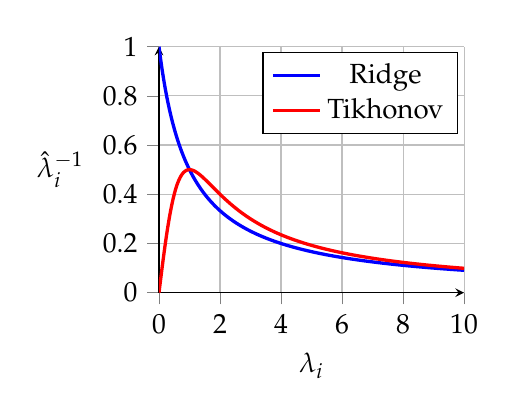
\begin{tikzpicture}
                \begin{axis}[xmin=0,xmax=10,ymin=0,width=0.45*\textwidth,grid,axis x line=left ,axis y line=left, tick align=outside,xlabel = $\lambda_i$,ylabel =$\hat{\lambda}_i^{-1}$,ylabel style={rotate=-90}]
                    \addplot+[very thick,mark=none,smooth,domain=0:10,samples=200] (\x,{1./(1.+\x)});
                    \addplot+[very thick,mark=none,smooth,domain=0:10,samples=200] (\x,{\x/(\x*\x + 1.)});
                    \addlegendentry{Ridge}
                    \addlegendentry{Tikhonov}
                \end{axis}
            \end{tikzpicture}
            \caption{Consequence of regularization on eigenvalues with $\tau=1$.\label{fig:eigenvalues}}
        \end{figure}


        In particular, the ridge regularization proposes to solve the problem in adding a small value $\tau$ to each eigenvalues of the covariance matrix. In our case, we choose to add the same constant for each class but it is not compulsory in a general case.

        Thus, in practice, we choose to use ridge regularization. To perform the regularization, the covariance matrix is decomposed with a diagonalization algorithm for symmetric matrices s.t. $\boldsymbol{\Sigma} = \mathbf{Q} \boldsymbol{\Lambda} \mathbf{Q}^t$ where $\boldsymbol{\Lambda}$ is the diagonal matrix of eigenvalues and $\mathbf{Q}$ is the matrix of associated eigenvectors. When the decomposition is available, the regularization is almost finished and the decision function is simply rewritten as follow

        \begin{align}
        \label{eq:decision-ridge}
            Q_c(\mathbf{x}) = - (\mathbf{x} - \boldsymbol{\mu}_c)^t \mathbf{Q}_c (\boldsymbol{\Lambda}_c + \tau \mathbf{I})^{-1} \mathbf{Q}_c^t (\mathbf{x} - \boldsymbol{\mu}_c) - \log (|\boldsymbol{\Sigma}_c + \tau \mathbf{I}|) + 2 \log (\pi_c) - d \log (2\pi),
        \end{align}
        where $\mathbf{I}$ is the identity matrix. It is to be noticed that $(\boldsymbol{\Lambda} + \tau \mathbf{I})$ is also a diagonal matrix and so the inverse is easily obtained in inverting each diagonal element of the matrix.

        \subsubsection{Implementation}

        The main steps of the training algorithm are summarized in Algorithm \ref{alg:ridge}. Indeed, before training the GMM model, a preliminary step is needed in order to determine a good value for the parameter $\tau$. A gridsearch is performed with a set of values $\mathcal{P}$ given by the user. To estimate the quality of the classification with a given $\tau$, one of the good classification criterion presented in Section~\ref{sec:criterion-rate} is used. As explained at the end of the same section, the classification rate is computed with a cross-validation process.

        A particularity of this regularization method is used to accelerate the gridsearch. More precisely, the two computationally costly step are the computation of the inverse and the determinant of the regularized covariance matrices and it is important to see that these operations can be performed only once to test all $\tau$. The covariance matrix is diagonalized before selecting $\tau$ and the eigenvalues and eigenvectors are stored and the regularized inverse and determinant can be update as follows
        \begin{align}
            \hat{\boldsymbol{\Sigma}}_c^{-1} &= \mathbf{Q}_c (\boldsymbol{\Lambda}_c + \tau \mathbf{I})^{-1} \mathbf{Q}_c^t, \nonumber\\
            \log (|\hat{\boldsymbol{\Sigma}}_c|) &= \log (|\boldsymbol{\Sigma}_c + \tau \mathbf{I}|) = \sum_{i=1}^{d} \log (\lambda_i + \tau).
            \label{eq:update-reg}
        \end{align}

        \begin{algorithm}
        \caption{Ridge regularization training steps\label{alg:ridge}}
        \begin{algorithmic}[1]
        \REQUIRE $\mathcal{S},k,\mathcal{P}$
        \STATE Learn GMM with $\mathcal{S}$
        \STATE Randomly cut $\mathcal{S}$ in $k$ subsets such as $\mathcal{S}_1 \cup \text{...} \cup \mathcal{S}_k = \mathcal{S}$ and $\mathcal{S}_i \cap \mathcal{S}_j = \emptyset$
        \FORALL{$\mathcal{S}_i$}
        \STATE Update GMM model for $i^{th}$ fold with Equations \ref{eq:update-cv1} and \ref{eq:update-cv2}
        \STATE Compute decomposition of covariance matrices of each class s.t. $\boldsymbol{\Sigma}_c = \mathbf{Q}_c \boldsymbol{\Lambda}_c \mathbf{Q}_c^t$
        \FORALL{$\tau \in \mathcal{P}$}
        \STATE Update inverse and logdet with Equations \ref{eq:update-reg}
        \STATE Estimate classification rate on $\mathcal{S}_i$ using Equation \ref{eq:decision-ridge}
        \ENDFOR
        \ENDFOR
        \STATE Average the classification rate over the $k$ folds
        \STATE Compute $\text{arg} \max_{\tau}$ of the classification rates to get the best parameter $\tau^*$
        \STATE Parametrize the GMM with $\tau^*$
        \end{algorithmic}
        \end{algorithm}

        Finally, another trick could used to optimize the gridsearch. As explained in Section~\ref{sec:update-cv}, it is possible to avoid the learning step on the $(k-1)$ fold and instead learn the model with the whole dataset and deduce the submodel used for cross-validation from the complete model and the mean vector and covariance matrix of the $k^{th}$ fold.

        As stated before, we choose to implement a basic ridge regression method and only the small improvement explained herebefore as been proposed. To the contrary, we choose in our study to focus more on a feature selection method named sequential forward features selection described in following section.

    \subsection{Features selection}
    \label{sec:selection}

    The objective of feature selection is to select a subset of variables to describe each sample and so to get rid of high dimensionality and its curse.

    Features selection algorithms may be divided into three types. The first type which called filter method is based uniquely on data analysis. Features are ranked according to a statistical analysis of the data. For example, the Principal Component Analysis (PCA) described in \cite{jimenez1998supervised} is a typical filter method and there is numerous other methods \cite{bruzzone1995extension}, \cite{biesiada2007feature}, \cite{demir2008phase}.

    The second sort are known as wrapper methods which can be seen as search method to determine the best set of variables for a given learning model. As exhaustive searches are out of question in a practical amount of time, numerous search strategies have been designed some optimal under particular hypothesis \cite{narendra1977branch} and other suboptimal but easier to set up \cite{whitney1971direct}, \cite{somol1999adaptive}. The advantage of such methods compare to filter methods is that they are dedicated to a particular model but on the other hand, as they require the training of multiple models to test various set of variables, they tend to be slower.

    The third type corresponds to the embedded method which do not separate the features selection process from the learning algorithm and allow interaction between the two processes. The basic example of such method is the decision tree algorithm in which a feature is selected for the creation of each node. Embedded methods also exist for other model, e.g. SVM \cite{guyon2002gene} \cite{weston2003use}.

    The selection method proposed in this work in a wrapper method associated to GMM models. It is important to underline that this method is a \emph{selection} method and not an \emph{extraction} method. It means the subset of variables obtained is composed of actual variables of the original set and not variables built as combination of several others as it is the case for example with PCA. This choice is made to assure an easier interpretation by the user of the obtained subset of variables.

    Thus, in order to set a wrapper method, we need a function to rank the various features which we define in Section~\ref{sec:criterion} and a search strategy. Two search algorithms are presented: the sequential forward features selection method (Section \ref{sec:forward-presentation}) and the sequential floating forward feature selection method (\ref{sec:floating-presentation}) the second being a more complex variation of the first.

        \subsubsection{Criterion function}
        \label{sec:criterion}

        Criterion functions aim to evaluate either a rate of good classification or the separability/similarity of class distributions. These functions are used to estimate which sets of variables are the best to represent data, to assure the separability of the classes and to perform classification. The choice of a criterion function is the choice of a way to compare sets of variables.

            \paragraph{Measures of good classification}
            \label{sec:criterion-rate}

            \hspace{0pt} \\
            As described in \cite{congalton2008assessing} (chapter 4), all this measures of good classification are based on an error matrix $M$ called confusion matrix which is defined so that $M_{ij}$ is the number of samples of class $i$ classified as class $j$. The confusion matrix allows the computation of several interesting values relatively to each class:
            \begin{itemize}
                \item the number of True Positive (TP) corresponding to good prediction;
                \item the number of True Negative (TN) corresponding to good classification of the other class;
                \item the number of False Negative (FN) corresponding to the samples of the class labeled as an other class;
                \item the number of False Positive (FP) corresponding to the samples wrongly classified as part of of this class.
            \end{itemize}
            Figure~\ref{fig:confusion} illustrates the definition of this values.

            \begin{figure}[!ht]
                \centering
                \begin{tabular}{c >{\bfseries}r @{\hspace{0.7em}}c @{\hspace{0.4em}}c @{\hspace{0.4em}}c @{\hspace{0.7em}}l}
                  \multirow{10}{*}{\parbox{1.1cm}{\bfseries\raggedleft Actual\\ value}} &
                    & \multicolumn{3}{c}{\bfseries Prediction outcome} \\
                  & & \bfseries $c_1$ & \bfseries $c_2$ & \bfseries $c_3$ \\
                  & $c_1'$ & \MyBox{True}{Positive} & \MyBox{False}{Negative} & \MyBox{False}{Negative} \\[2.4em]
                  & $c_2'$ & \MyBox{False}{Positive} & \MyBox{True}{Negative} & \MyBox{~}{~} \\[2.4em]
                  & $c_3'$ & \MyBox{False}{Positive} & \MyBox{~}{~} & \MyBox{True}{Negative}
                \end{tabular}
                \caption{Confusion matrix with TP, TN, FP and FN relatively to $c_1$}
                \label{fig:confusion}
            \end{figure}

            \noindent\underline{\bfseries Global indices:}

            \subparagraph{The overall accuracy} is simply the rate of the number of samples with the correct predicted label over the number of samples. This metric is easy to interpret but is biased in the case of unbalanced classes.

            \subparagraph{The Cohen's kappa} is a statistic which measures the probability of agreement between predictions and ground-truth. This metric tends to give an equal importance to each class.

            \subparagraph{The mean F1 score} is the average of the F1 score for each class and the F1 score is the harmonic mean of the precision (number of True Positive over True Positive plus False Positive) and the recall (number of True Positive over True Positive plus False Negative).

            \begin{align}
                \text{Overall Accuracy} &= \frac{\text{TP}}{n}. \\
                \text{Kappa} &= \frac{pa - pr}{1 - pr}.  \\
                \text{F1 Mean} &= \frac{2 \text{TP}}{2 \text{TP} + \text{FN} + \text{FP}}.
            \end{align}
            where TP stands for True Positive, FN for False Negative, FP for False Positive, $pa$ is the probability of agreement defined by $pa = Overall Accuracy$  and $pr$ the probability of random agreement defined by $pr = \sum_{c=1}^{C} \frac{TP_c}{FP_c} \frac{TP_c}{FN_c}$.

            In order to estimate classification rate, the GMM has to be trained and tested on separate datasets. In our case, we choose to use a cross-validation process over our training set. Thus, the training set is divided in k folds, then, the training is done with $(k-1)$ folds and the performances are estimated with the remaining fold. For more details about cross-validation, see \cite{opac-b1127878} (Chapter 7.10).

            \paragraph{Measures of similarity between distributions}

            \hspace{0pt} \\
            The second type of criterion functions is a measure of distance between two distributions. These measures are called divergence function and are defined so that, if we note $S$ a space of all probability distribution with same support, it verifies
            \begin{align*}
                &\forall (p,q) \in S, \text{Div}(p,q) \geq 0, \\
                &\text{Div}(p,q) = 0 \Leftrightarrow p = q.
            \end{align*}
            More specifically, we focus on two particular divergences: the Kullback–Leibler divergence and the Jeffries–Matusita distance. The advantage of these divergences is that they have a explicit expression in the case of Gaussian models. The simplification allows us to get rid of any integration calculus which could be a major problem when dealing with high-dimensional data.


            \subparagraph{The Kullback–Leibler divergence} measures the amount of information lost when the first distribution is approximated by the second one. The formal definition is
            \begin{equation}
                \text{Div}_{KL}(c_i,c_j) = \int_\mathbf{x} p(\mathbf{x}|c_i) \ln(\frac{p(\mathbf{x}|c_i)}{p(\mathbf{x}|c_j)}) d\mathbf{x}.
            \end{equation}
            And in the case of Gaussian model, it can be rewritten as follows
            \begin{align}
                \text{Div}_{KL}(c_i,c_j) = \frac{1}{2} \left( \text{Tr} (\boldsymbol{\Sigma}_{c_i}^{-1} \boldsymbol{\Sigma}_{c_j}) + (\boldsymbol{\mu}_{c_i} - \boldsymbol{\mu}_{c_j})^t \boldsymbol{\Sigma}_{c_i}^{-1} (\boldsymbol{\mu}_{c_i} - \boldsymbol{\mu}_{c_j}) - d + \log \left( \frac{|\boldsymbol{\Sigma}_{c_i}|}{|\boldsymbol{\Sigma}_{c_j}|} \right) \right),
            \end{align}
            where Tr is the trace operator and $d$ the dimension of the distribution.

            It can be noticed that the KL divergence is not symmetric, i.e. $\text{Div}_{KL}(c_i,c_j) \ne \text{Div}_{KL}(c_j,c_i)$, and so the symmetrized version is used to compute the criterion function. In the case of Gaussian model, the symmetrization induces the following simplification of the formula
            \begin{align}
                \text{SKL}_{ij} &=\text{Div}_{KL}(c_i,c_j) + \text{Div}_{KL}(c_j,c_i) \nonumber \\
                &= \frac{1}{2} \left( \text{Tr} (\boldsymbol{\Sigma}_{c_i}^{-1} \boldsymbol{\Sigma}_{c_j} + \boldsymbol{\Sigma}_{c_j}^{-1} \boldsymbol{\Sigma}_{c_i}) + (\boldsymbol{\mu}_{c_i} - \boldsymbol{\mu}_{c_j})^t (\boldsymbol{\Sigma}_{c_i}^{-1} + \boldsymbol{\Sigma}_{c_j}^{-1}) (\boldsymbol{\mu}_{c_i} - \boldsymbol{\mu}_{c_j}) - 2d \right).
            \end{align}

            Moreover, the divergence is computed between two classes and to obtain a unique value the weighted mean of divergence measures is taken
            \begin{equation}
                \text{C}_{SKL} = \sum_{i=1}^{C} \sum_{j=i + 1}^{C} \pi_{c_i} \pi_{c_j} \text{SKL}_{ij}.
            \end{equation}

            \subparagraph{The Bhattacharyya distance} is defined as follows
            \begin{equation}
                \text{B}_{ij} = - \ln \left( \int_\mathbf{x} \sqrt{p(\mathbf{x}|c_i) p(\mathbf{x}|c_j)} d\mathbf{x} \right).
            \end{equation}
            And in the case of Gaussian model:
            \begin{equation}
                \text{B}_{ij} = \frac{1}{8} (\boldsymbol{\mu}_i - \boldsymbol{\mu}_j)^t \left( \frac{\boldsymbol{\Sigma}_i + \boldsymbol{\Sigma}_j}{2} \right)^{-1} (\boldsymbol{\mu}_i - \boldsymbol{\mu}_j) + \frac{1}{2} \ln \left( \frac{|\boldsymbol{\Sigma}_i + \boldsymbol{\Sigma}_j|}{\sqrt{|\boldsymbol{\Sigma}_i| |\boldsymbol{\Sigma}_j|}} \right).
            \end{equation}

            \subparagraph{The Jeffries–Matusita distance} is a measure based on the Bhattacharyya distance but transformed in a way that the distance saturates if the separability between the two distribution increases. The JM distance is defined according to
            \begin{equation}
                \text{JM}_{ij} = \sqrt{ \int_\mathbf{x} \left[\sqrt{p(\mathbf{x}|c_i)} - \sqrt{p(\mathbf{x}|c_j)}\right]^2 d\mathbf{x} }.
            \end{equation}
            And the Jeffries–Matusita distance can be rewritten according to the Bhattacharyya distance
            \begin{equation}
                \text{JM}_{ij} = \sqrt{ 2 \{1 - \text{exp}[-B_{ij}]\} }.
            \end{equation}

            As for the KL divergence, a weighted mean of the distance between two classes is computed to aggregate the measures in a single value.

            \vspace{10 mm}

            According to \cite{bruzzone2009novel}, it is interesting to notice that the KL divergence increases quadratically with respect to the distance between the mean vectors of the class distributions whereas the measures of good classification we used asymptotically tends to one when distributions are perfectly separable. On the contrary, the JM distance tends to saturate as these measures of good classification.


        \subsubsection{Selection method}

            \paragraph{Sequential forward features selection}
            \label{sec:forward-presentation}

            The Sequential Forward Selection (SFS) starts with an empty set of selected features. Then it tests at each step for all the remaining features the value of a criterion function $J$ chosen among the ones presented in Section \ref{sec:criterion} when the feature is added to the pool of selected features. The feature that maximizes the criterion function is definitively added to the pool of selected features and it moves to the next iteration. The algorithm stops when a given number of variables \emph{maxVarNb} has been selected. The Algorithm~\ref{alg:sfs} presents the process in details.

            To summarize, the features are selected one by one and the set of selected features are never questioned. It results in a reasonable computational time but a suboptimal solution to the selection problem meaning that a better subset of variables could exist.

            \begin{algorithm}
            \caption{Sequential forward features selection\label{alg:sfs}}
            {\fontsize{10}{10}\selectfont
            \begin{algorithmic}[1]
            \REQUIRE $\mathcal{S},J,\text{maxVarNb}$
            \STATE $S=\emptyset$
            \STATE $F=\text{\{all variables\}}$
            \WHILE{$\text{card}(S) \leq maxVarNb$}
            \FORALL{$f_i \in F$}
            \STATE $R_i = J(\{S + f_i\})$
            \ENDFOR
            \STATE $j=\text{arg} \max_{i} R_i$
            \STATE $S = \{S + f_j\}$
            \STATE $F = F \setminus f_j$
            \ENDWHILE
            \RETURN $S$
            \end{algorithmic}
            }
            \end{algorithm}


            Figure~\ref{fig:expl_dataset} shows a toy dataset with 2 classes and 2 features. The projection of the Gaussian distribution learned for each class can be visualized on the corresponding axis. In this examples, each class has been generated given a Gaussian law.

            \begin{figure}[!ht]
                \centering
                \begin{tabular}{cc}
                    \includegraphics[width=0.5\textwidth]{Fig/example_case1.pdf} &
                    \includegraphics[width=0.5\textwidth]{Fig/example_case2.pdf} \\
                    {\bfseries{(a)}} & {\bfseries{(b)}} \\
                    \multicolumn{2}{c}{\includegraphics[width=0.5\textwidth]{Fig/example_case3.pdf}} \\
                    \multicolumn{2}{c}{{\bfseries{(c)}}} \\
                \end{tabular}
                \caption{Example datasets: {\bfseries{(a)}} 2 classes and 2 features but only one informative feature, {\bfseries{(b)}} same dataset with a reduced gap between means of informative feature, {\bfseries{(c)}} similar dataset with unbalanced classes (350/50 samples).\label{fig:expl_dataset}}
            \end{figure}

            In the cases of the example presented in Figure~\ref{fig:expl_dataset}, we compute the criterion functions described in \ref{sec:criterion} and summarize it in Table \ref{tab:expl_metric}. We can see that all the criterion functions are maximum with the feature 1 which makes sense because the projection of the learned Gaussian distribution effectively seems separable only for feature 1. So the algorithm will select the feature 1 as the best feature to perform classification. The case (c) also shows that the measures are robust to unbalanced classes except the overall accuracy which, as we can see, do not make much difference between the two features because of the imbalance.

            \begin{table}[!ht]
                \resizebox{\textwidth}{!}{%
                \begin{tabular}{l|r|r|r|r|r|r|r|r|r}
                     & \multicolumn{3}{c|}{Case a} & \multicolumn{3}{c|}{Case b} & \multicolumn{3}{c}{Case c} \\
                    \hline
                     & Feat 1 & Feat 2 & Feat 1+2 & Feat 1 & Feat 2 & Feat 1+2 & Feat 1 & Feat 2 & Feat 1+2 \\
                    \hline
                    Overall Accuracy          & 0.995 & 0.445 & 0.995 & 0.935 & 0.445 & 0.925 & 0.985 & 0.87 & 0.985 \\
                    Cohen's kappa             & 0.99  & -0.11 & 0.99  & 0.87  & -0.11 & 0.85  & 0.95  & 0    & 0.95 \\
                    F1-score mean             & 0.995 & 0.43  & 0.995 & 0.935 & 0.43  & 0.92  & 0.97  & 0.47 & 0.97 \\
                    KL divergence             & 13.04 & 0.25  & 13.44 & 3.48  & 0.25  & 3.77  & 2.66  & 0.12 & 2.79 \\
                    Jeffrey-Matusita distance & 0.35  & 0.19  & 0.35  & 0.31  & 0.19  & 0.32  & 0.16  & 0.09 & 0.16 \\
                \end{tabular}}
                \caption{Criterion functions values corresponding to Figure~\ref{fig:expl_dataset} dataset (50\% for training/50\% for testing).\label{tab:expl_metric}}
            \end{table}

            \paragraph{Sequential floating forward feature selection}
            \label{sec:floating-presentation}

            The Sequential Floating Forward Selection (SFFS) is actually based on two algorithms: the SFS described above and the Sequential Backward Selection (SBS). The SBS is the backward equivalent of SFS. The difference is that it starts with every features in the pool of selected features and tries at each step to remove the less significant one in term of the given criterion function.

            The SFFS works as the SFS but between each step of the SFS algorithm a backward selection is operated. At the end of the SBS step, the value of the criterion function is compared to the best value ever obtained with a set of features of the same size and if the new value is better the feature puts into question is effectively taken away and the next step is again a SBS but if the new value is not better the SBS step is forgotten and it moves to the next SFS step. The algorithm stops when a given number of features has been selected. The Algorithm~\ref{alg:sffs} sums up the method.

            This SFFS algorithm eventually tests more solutions than the SFS algorithm. The results are expected to be better but the trade-off is an increased computational time which is dependent on the complexity of the dataset.

            \begin{algorithm}
            \caption{Sequential floating forward features selection\label{alg:sffs}}
            {\fontsize{10}{10}\selectfont
            \begin{algorithmic}[1]
            \REQUIRE $\mathcal{S},J,\text{maxVar}$
            \STATE $S=\emptyset$
            \STATE $F=\text{\{all variables\}}$
            \STATE $k=0$
            \WHILE{Repeat till $S$ contained $\text{maxVar}$ variables}
            \FORALL{$f_i \in F$}
            \STATE $R_i = J(\{S{(k)} + f_i\})$
            \ENDFOR
            \STATE $j=\text{arg} \max_{i} R_i$
            \IF{$R_j \geq J(S^{(k+1)})$}
            \STATE $k=k+1$
            \ELSE
            \STATE $S^{(k+1)} = \{S{(k)} + f_i\}$
            \STATE $k=k+1$
            \STATE $\text{flag}=1$
            \WHILE{$k > 2 \text{ and } \text{flag}=1$}
            \FORALL{$f_i \in S^{(k)}$}
            \STATE $R_i = J(\{S{(k)}\setminus f_i\})$
            \ENDFOR
            \STATE $j=\text{arg} \max_{i} R_i$
            \IF{$R_j < J(S^{(k-1)})$}
            \STATE $S^{(k-1)} = \{S{(k)} \setminus f_i\}$
            \STATE $k=k-1$
            \ELSE
            \STATE $\text{flag}=0$
            \ENDIF
            \ENDWHILE
            \ENDIF
            \ENDWHILE
            \RETURN $S$
            \end{algorithmic}
            }
            \end{algorithm}


\section{Smart implementation}
\label{sec:implementation}

    \subsection{Statistical update rules}
    A major contribution of our work is the optimization in term of computational efficiency. More precisely, three steps of our method has been upgraded in order to reduce computational time. First of all, the GMM model is learned only once using samples. When a covariance matrix or a mean vector of a reduced set of variables is required, we get it from the global model learned at the beginning.

    Secondly, when a cross-validation is performed, we do not learn a submodel, i.e. a GMM model trained with $(n-1)$ folds, using the $(n-1)$ folds but, instead, we derive it from the global model and the covariance matrices and mean vectors of the fold used for validation for this given submodel. The process is described in details in Section~\ref{sec:update-cv}.

    Finally and most importantly, when variables are tested one by one during a selection step, costly operations are made when computing criterion functions for each variable especially the computation of the inverse of covariance matrices and its determinant. We manage to set up several update rules which allow us to compute this inverse and determinant only once to test all variables. These update rules are presented in Section~\ref{sec:update-crit}.

        \subsubsection{Update for cross validation}
        \label{sec:update-cv}

        Based on \cite{fauvel2015fast}, a method to accelerate the k-fold cross-validation process in the case of criterion functions based on correct classification measures was implemented. The idea is to estimate the GMM model with the whole training set and then, instead of training a model on $(k-1)$ folds, the complete model and the mean vector and the covariance matrix of the $k^{th}$ fold is used to derive the corresponding submodel.

        The following formulae can be obtained (details of calculation in Appendix \ref{app:cv_maj})
        \begin{prop}
            \label{eq:update-cv1}
            (CV mean update)
            \begin{equation*}
                \boldsymbol{\mu}_c^{n_c-\nu_c} = \frac{n_c \boldsymbol{\mu}_c^{n_c} - \nu_c \boldsymbol{\mu}_c^{\nu_c}}{n_c - \nu_c} \nonumber
            \end{equation*}
        \end{prop}
        \begin{prop}
            \label{eq:update-cv2}
            (CV covariance matrix update)
            \begin{equation*}
                \boldsymbol{\Sigma}_c^{n_c-\nu_c} = \frac{1}{n_c-\nu_c-1} ( (n_c-1) \boldsymbol{\Sigma}_c^{n_c} - (\nu_c-1) \boldsymbol{\Sigma}_c^{\nu_c} - \frac{n_c \nu_c}{(n_c-\nu_c)} (\boldsymbol{\mu}_c^{\nu_c}-\boldsymbol{\mu}_c^{n_c})(\boldsymbol{\mu}_c^{\nu_c}-\boldsymbol{\mu}_c^{n_c})^t) \nonumber
            \end{equation*}
        \end{prop}
        where $\nu_c$ is the number of samples of class $c$ removed from the set, $\boldsymbol{\mu}_c^{n_c}$ the mean vector estimated with this $\nu_c$ samples and $\boldsymbol{\Sigma}_c^{\nu_c}$ the covariance matrix estimated with this $\nu_c$ samples.

        Additionally, the update of the GMM model is the occasion to precompute and store the constant $2 \log (\pi_c)$ which is a term of the decision function constant for a given training set.

        \subsubsection{Criterion function computation}
        \label{sec:update-crit}

        As explained earlier, at each iteration the SFS and SFFS algorithms compute the value of a criterion function for every possible set of features composed of the selected ones augmented by one of the remaining features. One of the main achievements of this work is to reduce the computational time needed to compute the criterion function of augmented sets.

        We note $\boldsymbol{\Sigma}^{(k-1)}$ a covariance matrix of the $(k-1)^{th}$ iteration, i.e., a covariance of the selected features and $\boldsymbol{\Sigma}^{(k)}$ the corresponding covariance matrix at the $k^{th}$ iteration, i.e., the covariance of the augmented set. Then, the inverse of the covariance matrix $(\boldsymbol{\Sigma}^{(k)})^{-1}$, the quadratical term $(\mathbf{x}^{(k)})^t (\boldsymbol{\Sigma}^{(k)})^{-1} \mathbf{x}^{(k)}$ and the determinant $\log |\boldsymbol{\Sigma}^{(k)}|$ can be expressed in function of terms of the $(k-1)^{th}$ iteration. These calculi use the fact that the covariance matrix is a positive definite symmetric matrix to simplify formulae using matrices defined by blocks. These update rules are summed up hereafter and are available in \cite{webb2003statistical} (chapter 9.2).

        In order to easily understand which terms are available and which ones needs to be computed, we choose to set in green in the update rules the terms already computed.

        As $\boldsymbol{\Sigma}^{(k)}$ is a positive definite symmetric matrix, we can use the following notation
        \begin{equation*}
            \boldsymbol{\Sigma}^{(k)} =
            \bigg[\begin{array}{cc}
            \boldsymbol{\Sigma}^{(k-1)} & \mathbf{u}      \\
            \mathbf{u}^t          & \sigma_{kk} \\
            \end{array}\bigg],
        \end{equation*}
        where $\mathbf{u}$ is the $k^{th}$ column of the matrix without the diagonal element i.e. $\mathbf{u}_{i} = \boldsymbol{\Sigma}^{(k)}_{i,k}$ with $i \in [1,k-1]$.

        Using the formula of the inverse of a block matrix, the following formula expressing $(\boldsymbol{\Sigma}^{(k)})^{-1}$ in function of $(\boldsymbol{\Sigma}^{(k-1)})^{-1}$ is obtained
        \begin{prop}
        \label{eq:update-inv}
            (Forward update rule for inverse of covariance matrix)
            \begin{equation*}
                \fbox{$
                (\boldsymbol{\Sigma}^{(k)})^{-1} =
                \bigg[\begin{array}{cc}
                \textcolor{OliveGreen}{(\boldsymbol{\Sigma}^{(k-1)})^{-1}} + \frac{1}{\alpha} \textcolor{OliveGreen}{(\boldsymbol{\Sigma}^{(k-1)})^{-1}} \mathbf{u} \mathbf{u}^t \textcolor{OliveGreen}{(\boldsymbol{\Sigma}^{(k-1)})^{-1}} & - \frac{1}{\alpha} \textcolor{OliveGreen}{(\boldsymbol{\Sigma}^{(k-1)})^{-1}} \mathbf{u} \\
                - \frac{1}{\alpha} \mathbf{u}^t \textcolor{OliveGreen}{(\boldsymbol{\Sigma}^{(k-1)})^{-1}}                                                                          & \frac{1}{\alpha}                  \\
                \end{array}\bigg]
                $}
            \end{equation*}
        \end{prop}
        where $ \alpha = \sigma_{kk} - \mathbf{u}^t \textcolor{OliveGreen}{(\boldsymbol{\Sigma}^{(k-1)})^{-1}} \mathbf{u} $.

        To insist again on the advantage given by this update rules, it means that, if we want to select a variable among one hundred, instead of computing one hundred times $(\boldsymbol{\Sigma}^{(k)})^{-1}$, we will compute $(\boldsymbol{\Sigma}^{(k-1)})^{-1}$ once and then with a few matrix multiplications and sums we can get the hundred inverses and so save a lot of processing time.

        In the case of a backward step in SFFS algorithm, we need to invert the formula in order to compute $(\boldsymbol{\Sigma}^{(k-1)})^{-1}$ knowing $(\boldsymbol{\Sigma}^{(k)})^{-1}$. So if we note
        \begin{equation*}
            (\boldsymbol{\Sigma}^{(k)})^{-1} =
            \bigg[\begin{array}{cc}
            \mathbf{A}   & \mathbf{v} \\
            \mathbf{v}^t & \frac{1}{\alpha} \\
            \end{array}\bigg].
        \end{equation*}
        Thus, the update rule becomes
        \begin{prop}
            (Backward update rule for inverse of covariance matrix)
            \begin{equation*}
                \fbox{$(\boldsymbol{\Sigma}^{(k-1)})^{-1} = \textcolor{OliveGreen}{\mathbf{A}} - \alpha \mathbf{v} \mathbf{v}^t$}
            \end{equation*}
        \end{prop}

        \begin{proof}
            \begin{align*}
                \mathbf{A} - \alpha \mathbf{v} \mathbf{v}^t
                &= (\boldsymbol{\Sigma}^{(k-1)})^{-1} + \frac{1}{\alpha} (\boldsymbol{\Sigma}^{(k-1)})^{-1} \mathbf{u} \mathbf{u}^t (\boldsymbol{\Sigma}^{(k-1)})^{-1} - \alpha (- \frac{1}{\alpha} (\boldsymbol{\Sigma}^{(k-1)})^{-1} \mathbf{u}) (- \frac{1}{\alpha} \mathbf{u}^t (\boldsymbol{\Sigma}^{(k-1)})^{-1})) \\
                &= (\boldsymbol{\Sigma}^{(k-1)})^{-1}
            \end{align*}
        \end{proof}

        A formula can also be deduced for the quadratical term of the decision function. If we note $(\mathbf{x}^{(k)})^t = \left[\begin{array}{cc} (\mathbf{x}^{(k-1)})^t   & x^k \end{array}\right]$, we get the following proposition
        \begin{prop}
        \label{eq:update-quad}
            (Update rule for quadratical term)
            \begin{equation*}
                \fbox{$(\mathbf{x}^{(k)})^t (\boldsymbol{\Sigma}^{(k)})^{-1} \mathbf{x}^{(k)} = \textcolor{OliveGreen}{(\mathbf{x}^{(k-1)})^t (\boldsymbol{\Sigma}^{(k-1)})^{-1} \mathbf{x}^{(k-1)}} + \alpha ( \left[\begin{array}{cc} \mathbf{v}^t & \frac{1}{\alpha} \end{array}\right] \mathbf{x}^{(k)} )^2$}
            \end{equation*}
        \end{prop}

        \begin{proof}
            \begin{align*}
                (\mathbf{x}^{(k)})^t (\boldsymbol{\Sigma}^{(k)})^{-1} \mathbf{x}^{(k)}
                &= \left[\begin{array}{cc} (\mathbf{x}^{(k-1)})^t   & x_k \end{array}\right]
                \left[\begin{array}{cc}
                \mathbf{A}   & \mathbf{v} \\
                \mathbf{v}^t & \frac{1}{\alpha}
                \end{array}\right]
                \left[\begin{array}{c} \mathbf{v} \\ x_k \end{array}\right] \\
                &= \left[\begin{array}{cc} (\mathbf{x}^{(k-1)})^t \mathbf{A} + x_k \mathbf{v}^t & (\mathbf{x}^{(k-1)})^t \mathbf{v} + \frac{x_k}{\alpha} \end{array}\right]
                \left[\begin{array}{c} \mathbf{v} \\ x_k \end{array}\right] \\
                &= (\mathbf{x}^{(k-1)})^t \mathbf{A} \mathbf{x}^{(k-1)} + x_k \mathbf{v}^t \mathbf{x}^{(k-1)} + (\mathbf{x}^{(k-1)})^t \mathbf{v} x_k + \frac{(x_k)^2}{\alpha} \\
                &= (\mathbf{x}^{(k-1)})^t ((\boldsymbol{\Sigma}^{(k-1)})^{-1} + \frac{1}{\alpha} (\boldsymbol{\Sigma}^{(k-1)})^{-1} \mathbf{u} \mathbf{u}^t (\boldsymbol{\Sigma}^{(k-1)})^{-1}) \mathbf{x}^{(k-1)}
                   + 2 x_k \mathbf{v}^t \mathbf{x}^{(k-1)} + \frac{(x_k)^2}{\alpha} \\
                &= (\mathbf{x}^{(k-1)})^t ((\boldsymbol{\Sigma}^{(k-1)})^{-1} + \alpha \mathbf{v} \mathbf{v}^t) \mathbf{x}^{(k-1)}
                   + 2 x_k \mathbf{v}^t \mathbf{x}^{(k-1)} + \frac{(x_k)^2}{\alpha} \\
                &= (\mathbf{x}^{(k-1)})^t (\boldsymbol{\Sigma}^{(k-1)})^{-1} \mathbf{x}^{(k-1)} + \alpha ( (\mathbf{x}^{(k-1)})^t \mathbf{v} \mathbf{v}^t \mathbf{x}^{(k-1)}
                   + 2 \frac{x_k}{\alpha} \mathbf{v}^t \mathbf{x}^{(k-1)} + \frac{(x_k)^2}{\alpha^2}) \\
                &= (\mathbf{x}^{(k-1)})^t (\boldsymbol{\Sigma}^{(k-1)})^{-1} \mathbf{x}^{(k-1)} + \alpha ( (\mathbf{x}^{(k-1)})^t \mathbf{v} + \frac{x_k}{\alpha} )^2 \\
                &= (\mathbf{x}^{(k-1)})^t (\boldsymbol{\Sigma}^{(k-1)})^{-1} \mathbf{x}^{(k-1)} + \alpha ( \left[\begin{array}{cc} \mathbf{v}^t & \frac{1}{\alpha} \end{array}\right] \mathbf{x}^{(k)} )^2
            \end{align*}
        \end{proof}

        Finally, using the formula of the determinant of a block matrix and after taking the log, we obtain
        \begin{prop}
        \label{eq:update-log}
            (Update rule for logdet)
            \begin{equation*}
                \fbox{$\log \left(|\boldsymbol{\Sigma}^{(k)}|\right) = \textcolor{OliveGreen}{\log \left(|\boldsymbol{\Sigma}^{(k-1)}|\right)} + \log \alpha$}
            \end{equation*}
        \end{prop}

        Now using all update rules, criterion functions can be rewritten as follows
        \begin{align}
        \label{eq:q-update}
            Q(\mathbf{x}) = &- \textcolor{OliveGreen}{(\mathbf{x}^{(k-1)} - \boldsymbol{\mu}^{(k-1)})^t (\boldsymbol{\Sigma}^{(k-1)})^{-1} (\mathbf{x}^{(k-1)} - \boldsymbol{\mu}^{(k-1)})} \nonumber \\
            &- \alpha \left( \left[\begin{array}{cc} \mathbf{v}^t & \frac{1}{\alpha} \end{array}\right] (\mathbf{x}^{(k)} - \boldsymbol{\mu}^{(k)}) \right)^2 \nonumber \\
            &- \textcolor{OliveGreen}{\log \left(|\boldsymbol{\Sigma}^{(k-1)}|\right)} - \log \alpha  + \textcolor{OliveGreen}{2 \log (\pi_c)} + \textcolor{OliveGreen}{k \log(2 \pi)};
        \end{align}

        \begin{align}
        \label{eq:skl-update}
            \text{SKL}_{ij} = &\frac{1}{2} \biggl( \text{Tr} \left((\boldsymbol{\Sigma}_{c_i}^{(k)})^{-1} \boldsymbol{\Sigma}_{c_j}^{(k)} + (\boldsymbol{\Sigma}_{c_j}^{(k)})^{-1} \boldsymbol{\Sigma}_{c_i}^{(k)}\right)
            + \textcolor{OliveGreen}{(\boldsymbol{\mu}_{c_i}^{(k-1)} - \boldsymbol{\mu}_{c_j}^{(k-1)})^t ((\boldsymbol{\Sigma}_{c_i}^{(k-1)})^{-1} + (\boldsymbol{\Sigma}_{c_j}^{(k-1)})^{-1}) (\boldsymbol{\mu}_{c_i}^{(k-1)} - \boldsymbol{\mu}_{c_j}^{(k-1)})} \nonumber \\
            &+ \alpha ( \left[\begin{array}{cc} \mathbf{v_i}^t & \frac{1}{\alpha_i} \end{array}\right] (\boldsymbol{\mu}_{c_i}^{(k)} - \boldsymbol{\mu}_{c_j}^{(k)}) )^2
            + \alpha ( \left[\begin{array}{cc} \mathbf{v_j}^t & \frac{1}{\alpha_j} \end{array}\right] (\boldsymbol{\mu}_{c_i}^{(k)} - \boldsymbol{\mu}_{c_j}^{(k)}) )^2
            - \textcolor{OliveGreen}{2k} \biggr),
        \end{align}
        with $(\boldsymbol{\Sigma}_{c_i}^{(k)})^{-1}$ computed with Proposition~\ref{eq:update-inv};

        \begin{align}
        \label{eq:jm-update}
            \text{B}_{ij} = &\textcolor{OliveGreen}{\frac{1}{4} (\boldsymbol{\mu}_i^{(k-1)} - \boldsymbol{\mu}_j^{(k-1)})^t ( \boldsymbol{\tilde{\Sigma}}^{(k-1)} )^{-1} (\boldsymbol{\mu}_i^{(k-1)} - \boldsymbol{\mu}_j^{(k-1)})} + \frac{1}{4} \tilde{\alpha} ( \left[\begin{array}{cc} \mathbf{\tilde{v}}^t & \frac{1}{\tilde{\alpha}} \end{array}\right] (\boldsymbol{\mu}_{i}^{(k)} - \boldsymbol{\mu}_{j}^{(k)}) )^2 \nonumber \\
            &+ \textcolor{OliveGreen}{\frac{1}{2} \ln \left( \frac{|\boldsymbol{\tilde{\Sigma}}^{(k-1)}|}{\sqrt{|\boldsymbol{\Sigma}_i^{(k-1)}| |\boldsymbol{\Sigma}_j^{(k-1)}|}} \right)} + \frac{1}{2} \ln \left( \frac{\tilde{\alpha}}{\sqrt{\alpha_i \alpha_j}} \right),
        \end{align}
        where $\boldsymbol{\tilde{\Sigma}} = \boldsymbol{\Sigma}_i + \boldsymbol{\Sigma}_j$.

        The Algorithm~\ref{alg:sffs-update} illustrates the optimization of the Algorithm~\ref{alg:sffs} developed using these formulae.

    \subsubsection{Computational issues}

    During an iteration of the selection algorithm, it still needs to invert the covariance matrix of the previous iteration. In order to so, we choose to perform a decomposition in eigenvalues and eigenvectors using algorithm specific for symmetric matrices. In other words, we find $\boldsymbol{\Lambda}$ the diagonal matrix of eigenvalues and $\mathbf{Q}$ the matrix of eigenvectors s.t. $\boldsymbol{\Sigma} = \mathbf{Q} \boldsymbol{\Lambda} \mathbf{Q}^t$.

    This decomposition has several advantages. First, it is very simple to compute the determinant once the eigenvalues are available because the determinant is equal to the product of these values. Secondly, it is possible to check the eigenvalues and so to assure a better computational stability. Due to the curse of dimensionality, the covariance matrix is sometimes badly conditioned and the result is that some eigenvalues are really small (below computational precision). The decomposition helps us to check their actual values and if they are below EPS\_FLT which is the machine maximum precision for a float, we set these eigenvalues to EPS\_FLT. For the same reason, the constant $\alpha$ used in update rules is also thresholded to EPS\_FLT. Algorithm~\ref{alg:sffs-update} details when computational stability is checked. We choose to underline the steps added compared to Algorithm~\ref{alg:sffs}.

    \begin{algorithm}
    \caption{Sequential floating forward features selection with updates\label{alg:sffs-update}}
    {\fontsize{8}{8}\selectfont
    \begin{algorithmic}[1]
    \REQUIRE $\mathcal{S},J,\text{maxVar}$
    \STATE $S=\emptyset$
    \STATE $F=\text{\{all variables\}}$
    \STATE $k=0$
    \WHILE{Repeat till $S$ contained $\text{maxVar}$ variables}
    \STATE \underline{Diagonalize $\boldsymbol{\Sigma}^{(k-1)} = \mathbf{Q} \boldsymbol{\Lambda} \mathbf{Q}^t$}
    \STATE \underline{\bfseries{for all} $\lambda_i$ \bfseries{do} $\lambda_i = \min (\text{EPS\_FLT},\lambda_i)$}
    \STATE \underline{Precompute $(\boldsymbol{\Sigma}^{(k-1)})^{-1}$, $(\mathbf{x}^{(k-1)} - \boldsymbol{\mu}^{(k-1)})^t (\boldsymbol{\Sigma}^{(k-1)})^{-1} (\mathbf{x}^{(k-1)} - \boldsymbol{\mu}^{(k-1)})$ and $\log \left(|\boldsymbol{\Sigma}^{(k-1)}|\right)$} \underline{using Propositions \ref{eq:update-inv}, \ref{eq:update-quad} and \ref{eq:update-log}}
    \FORALL{$f_i \in F$}
    \STATE \underline{Compute update constant $\alpha$}
    \STATE \underline{$\alpha = \min (\text{EPS\_FLT},\alpha)$}
    \STATE $R_i = J(\{S{(k)} + f_i\})$ \underline{using Equations \ref{eq:q-update}, \ref{eq:skl-update} or \ref{eq:jm-update}}
    \ENDFOR
    \STATE $j=\text{arg} \max_{i} R_i$
    \IF{$R_j \geq J(S^{(k+1)})$}
    \STATE $k=k+1$
    \ELSE
    \STATE $S^{(k+1)} = \{S{(k)} + f_i\}$
    \STATE $k=k+1$
    \STATE $\text{flag}=1$
    \WHILE{$k > 2 \text{ and } \text{flag}=1$}
    \STATE \underline{Diagonalize $\boldsymbol{\Sigma}^{(k-1)} = = \mathbf{Q} \boldsymbol{\Lambda} \mathbf{Q}^t$}
    \STATE \underline{\bfseries{for all} $\lambda_i$ \bfseries{do} $\lambda_i = \min (\text{EPS\_FLT},\lambda_i)$}
    \STATE \underline{Precompute $(\boldsymbol{\Sigma}^{(k-1)})^{-1}$, $(\mathbf{x}^{(k-1)} - \boldsymbol{\mu}^{(k-1)})^t (\boldsymbol{\Sigma}^{(k-1)})^{-1} (\mathbf{x}^{(k-1)} - \boldsymbol{\mu}^{(k-1)})$ and $\log \left(|\boldsymbol{\Sigma}^{(k-1)}|\right)$} \underline{using Propositions \ref{eq:update-inv}, \ref{eq:update-quad} and \ref{eq:update-log}}
    \FORALL{$f_i \in S^{(k)}$}
    \STATE \underline{Compute update constant $\alpha$}
    \STATE \underline{$\alpha = \min (\text{EPS\_FLT},\alpha)$}
    \STATE $R_i = J(\{S{(k)}\setminus f_i\})$ \underline{using Equations \ref{eq:q-update}, \ref{eq:skl-update} or \ref{eq:jm-update}}
    \ENDFOR
    \STATE $j=\text{arg} \max_{i} R_i$
    \IF{$R_j < J(S^{(k-1)})$}
    \STATE $S^{(k-1)} = \{S{(k)} \setminus f_i\}$
    \STATE $k=k-1$
    \ELSE
    \STATE $\text{flag}=0$
    \ENDIF
    \ENDWHILE
    \ENDIF
    \ENDWHILE
    \RETURN $S$
    \end{algorithmic}
    }
    \end{algorithm}

    \subsection{Implementation of the Orfeo Toolbox module}
    \label{sec:otb-implememtation}

    After the calibration of the algorithm with a Python implementation, we aim to realize a C++ implementation of this selection method. And, to make it easily available, we choose to develop a remote module for the Orfeo Toolbox (OTB) designed by the CNES. The current section describes this C++ implementation.

        \subsubsection{Integration in Orfeo Toolbox}

        The Orfeo Toolbox is an open-source library for remote sensing image processing. This library allows developers to code external modules and make them available to the community. It is to note that the toolbox already implements several classifiers inherited mostly from OpenCV. Nevertheless, the GMM classifier currently in place is not robust to high dimensionality (see Section~\ref{sec:exp-otb}) and that's why we choose to implement our own model.

        The module we developed is available on Github \footnote{\url{https://github.com/Laadr/otbExternalFastFeaturesSelection}} and is actually a fork of the template for remote module furnished by OTB developers.

        \subsubsection{Code structure}

        \begin{figure}[!ht]
            \centering
            \begin{tikzpicture}
                \begin{umlpackage}{otb}
                    \umlclass[template={InType,LabType}, x=4.5]{MachineLearningModel}{
                        m\_InputListSample : ListSample<InType>*\\
                        m\_TargetListSample : ListSample<LabType>*
                    }{
                        \umlvirt{Train() : void} \\
                        \umlvirt{Predict() : LabType} \\
                        \umlvirt{Save() : void} \\
                        \umlvirt{Load() : void} \\
                        \umlvirt{CanReadFile() : bool} \\
                        \umlvirt{CanWriteFile() : bool}
                    }
                \end{umlpackage}

                \begin{umlpackage}{otbExternalFastFeaturesSelection}
                    \umlclass[template={InType,LabType}, y=-8]{GMMMachineLearningModel}{
                        m\_ClassNb : unsigned\\
                        m\_FeatNb : unsigned\\
                        m\_Proportion : vector<double>\\
                        m\_NbSpl : vector<unsigned>\\
                        m\_Means : vector<vnl\_vector>\\
                        m\_Covariances : vector<vnl\_matrix>\\
                        m\_Tau : RealType\\
                        m\_RateGridsearch : vector<RealType>\\
                        m\_EigenValues : vector<vnl\_vector>\\
                        m\_Q : vector<vnl\_matrix>\\
                        m\_LambdaQ : vector<vnl\_matrix>\\
                        m\_CstDecision : vector<RealType>
                    }{
                        SetTau() : void\\
                        TrainTau() : void\\
                        Decomposition() : void\\
                        Train() : void\\
                        Predict() : LabType\\
                        Save() : void\\
                        Load() : void\\
                        CanReadFile() : bool\\
                        CanWriteFile() : bool
                    }
                    \umlclass[template={InType,LabType}, x=8.5, y=-8]{GMMSelectionMachineLearningModel}{
                        m\_VarNbPrediction : int \\
                        m\_EnableOptimalSet : bool \\
                        m\_SelectedVar : vector<int>\\
                        m\_BestSets : vector<vector<int>> \\
                        m\_CriterionBestValues : vector<RealType> \\
                        m\_SubMeans :  vector<vnl\_vector> \\
                        m\_Logprop : vector<RealType> \\
                        m\_SubmodelCv : vector<ModelType> \\
                        m\_Fold : vector<ListSample*>
                    }{
                        Selection() : void\\
                        ForwardSelection() : void\\
                        FloatingForwardSelection() : void\\
                        ComputeClassifRate() : void\\
                        ComputeJM() : void\\
                        ComputeDivKL() : void\\
                        Train() : void\\
                        Predict() : LabType\\
                        Save() : void\\
                        Load() : void\\
                    }
                \end{umlpackage}

                \umlinherit[geometry=-|,anchor1=10]{GMMMachineLearningModel}{MachineLearningModel}
                \umlinherit[geometry=|-]{GMMSelectionMachineLearningModel}{GMMMachineLearningModel}
            \end{tikzpicture}
            \caption{UML digram of OTB remote module.\label{fig:uml}}
        \end{figure}

        Even if a GMM classifier inherited from Opencv library is already available in the OTB, we choose to implement our own version of a GMM classifier in a class named \emph{GMMMachineLearningModel} in order to assure better performance in term of computational time. The second step is to implement a subclass of the GMM classifier including the features selection method.

        The \emph{GMMMachineLearningModel} class inherits from the OTB class \emph{MachineLearningModel} which is a basic class used for all classifier in the OTB. The \emph{MachineLearningModel} class enables the management of a list of samples used for training and also declares the virtual methods inherited: \emph{Train()}, \emph{Predict()}, \emph{Save()}, \emph{Load()}, \emph{CanReadFile()}, \emph{CanWriteFile()}.

        The \emph{GMMMachineLearningModel} class implements all these virtual methods. The \emph{Train()} aims to train the classifier using a list of samples set as a member of the class. Then, it is possible to use the method \emph{Predict()} to classify a sample and optional get the confidence in the prediction. The methods \emph{Save()} and \emph{Load()} obviously are used to save and load a trained model. And, finally, \emph{CanReadFile()} and \emph{CanWriteFile()} state the validity of a GMM model file.

        In addition to these inherited methods, two noticeable methods are implemented. The \emph{Decomposition()} method perform a decomposition of a symmetric matrix in eigenvalues and eigenvectors using a function of the VNL library. It is to notice that this method check the value of the extracted eigenvalues and minor them to EPSILON\_FLT (or EPSILON\_DBL) which corresponds to computational precision.  The idea is to limit computational instability when parameters are badly-estimated due to an insufficient amount of training samples. The second interesting method is \emph{TrainTau()} which concerns the ridge regularization. Given a set of possible regularization constant $\tau$, this method selects the most efficient value in estimating classification rate with cross-validation.

        In term of members, the \emph{GMMMachineLearningModel} includes:
        \begin{itemize}
            \item 6 variables describing the model: the number of class, the number of features, the proportion of each class in the training set, the number of samples in each class, the mean vectors of each class and finally the covariance matrices of each class;
            \item 1 optional meta-parameter: the regularization value $\tau$ for ridge regularization;
            \item 1 variable the result of tau selection (classification rate for each tau);
            \item 4 precomputed terms used for prediction: eigenvalues of covariance matrices, eigenvectors of covariance matrices, 2 other terms.
        \end{itemize}

        To implement the selection algorithm, a new class \emph{GMMSelectionMachineLearningModel} inheriting from \emph{GMMMachineLearningModel} is defined. This class keeps the same six methods inherited from \emph{MachineLearningModel} but reimplements \emph{Predict()} to predict with a reduced set of features and  \emph{Save()}/\emph{Load()} to use a second file to handle the results of the selection.

        The other methods available in class \emph{GMMSelectionMachineLearningModel} are used to perform the selection algorithms presented in Section \ref{sec:gmm-hd}. The method \emph{Selection()} aims to set the various parameter of the selection and then calls either the \emph{ForwardSelection()} method to use forward feature selection or the \emph{FloatingForwardSelection()} method to use SFFS. Then, 3 different methods are used to evaluate criterion functions during selection. Given a pool of variables available for selection, these functions evaluate the criterion functions for all the possible augmented set. The \emph{ComputeJM()} method is used for Jeffries-Matusita distance, \emph{ComputeDivKL()} for Kullback–Leibler divergence and \emph{ComputeClassifRate()} for the three good classification criteria. It is to notice that the good classification criteria are evaluated using cross-validation.

        Several new members are defined in the \emph{GMMSelectionMachineLearningModel} class:
        \begin{itemize}
            \item 2 meta-parameters: one to specify the number of variables to use for prediction and one to enable the process to automatically set the previous meta-parameter to the number maximizing the criterion function;
            \item 3 variables describing the results of selection: the set to use for prediction, the evolution of criterion function at each iteration and the best sets for each iteration;
            \item 2 variables used for cross-validation: the set of submodels and the folds of samples;
            \item 2 precomputed terms used for prediction.
        \end{itemize}

        All the code structure is summarized in the UML diagram displayed in Figure~\ref{fig:uml}.

        \subsubsection{Applications}

        In order to provide an easy way to use the developed algorithm, we finally develop OTB application. These application allows the user to use and parametrize the algorithm from command line. Three applications are built.

        The application \emph{otbcli\_TrainGMMApp} creates and trains a model from class \emph{GMMMachineLearningModel} and the application \emph{otbcli\_TrainGMMSelectionApp} same for a model of class \emph{GMMSelectionMachineLearningModel}. These two applications use a raster image and shapefile with groundtruth as input and create a model file.

        The last application \emph{otbcli\_PredictGMMApp} takes a raster image as input and a model file and perform classification of the image. It generates a classification map in an image file and optionally a confidence map. An other application is available in the OTB to compute classification rate from the image and a groundtruth file.

\section{Experimental results}
\label{sec:test}

    \subsection{Test: GMM algorithm variations}
    \label{sec:gmm-results}
    In this section, we discuss the results of the features selection method. The forward selection and the floating forward selection are compared and the results with the different criterion function are also discussed. All the experimentation has been conducted with a dataset presented in the next subsection.

        \subsubsection{Aisa dataset}
        \label{sec:aisa}
        The Aisa dataset has been acquired by the AISA Eagle sensor during a flight campaign over Heves, Hungary. It contains 252 bands ranging from 395 to 975 nm. 16 classes have been defined for a total of 361,971 referenced pixels. Figure~\ref{fig:aisa} shows one channel of the multispectral image and the shapefile representing groundtruth and Table \ref{tab:aisa} presents the repartition of the various classes.

        \begin{figure}[!ht]
            \centering
            \begin{tabular}{cc}
                \includegraphics[width=0.5\textwidth]{Fig/aisa.png} &
                \includegraphics[width=0.5\textwidth]{Fig/aisa_gt.png} \\
                {\bfseries{(a)}} & {\bfseries{(b)}} \\
            \end{tabular}
            \caption{Aisa dataset: {\bfseries{(a)}} a single band of the image, {\bfseries{(b)}} groundtruth.\label{fig:aisa}}
        \end{figure}

        \begin{table}[!ht]
            \centering
            \begin{tabular}[b]{lc}\hline
              Class & Number of samples \\ \hline
              Winter wheat & 136,524 \\
              Sunflower & 61,517 \\
              Green fallow last year treatment & 30,197 \\
              Alfalfa & 17,626 \\
              Maize & 18,278 \\
              Millet & 7,199 \\
              Broadleaved forest & 10,746 \\
              Meadow & 23,283 \\
              Winter barley & 2,799 \\
              Reed & 4,222 \\
              Water course & 4,773 \\
              Rape & 26,566 \\
              Green fallow with shrub & 9,272 \\
              Green fallow last year treated & 3,426 \\
              Pasture & 2,107 \\
              Oat & 3,436 \\ \hline
            \end{tabular}
            \caption{table}{Repartition of classes in Aisa dataset.\label{tab:aisa}}
        \end{table}

        \subsubsection{Experimental results}

        For the results discussed in this section, the selection process was repeated 20 times with each time a different training set and the classification rate and time processing presented hereafter are the means over these 20 trials. We choose to present the results using Cohen's kappa but the same results have been obtained when we look at the mean of F1-scores.

        % discuss evolution of classif rate with nb of selected var
        Figure~\ref{fig:res-1} corresponds to the evolution of the classification rate expressed with Cohen's kappa in function of the number of selected variables. We observe that at first the classification rate rapidly increase before stabilizing and then slowly decrease. This is the typical behavior expected when using features selection and a GMM classifier and it illustrates the Hughes phenomenon \cite{hughes1968mean} which states that with a given number of samples, prediction accuracy first increases with dimensionality but then decays when the complexity is higher than some optimum value. In our particular case, $\frac{d(d+3)}{2}$ parameters have to be estimated. With $d=13$, it means 104 parameters and we use in this example 100 samples by class. Figure~\ref{fig:res-1} confirms this theoretical limit, as we can see, when the number of features is higher than 13, the classification rate actually becomes to decrease. In practice, we want to use the number of variables which maximizes the classification rate even if the maximum is not always easily found for example because of local maxima.


        \begin{figure}[!ht]
            \centering
            \includegraphics[width=0.5\textwidth]{Fig/aisa_trials_20_JM_fctvarnb.pdf}
            \caption{Classification results averaged on 20 trials using forward selection and Jeffries-Matusita distance as criterion with 100 samples by class in training set.\label{fig:res-1}}
        \end{figure}


        % discuss evolution with training set size
        It is also interesting to confirm the influence of the size of the training set. From Figure~\ref{fig:setsize}, we see that, either with an equalized training set or with a proportional training set, the classification rate is obviously better with more samples and also that the maximum is reached with more selected variables which means that more samples allows to evaluate more precisely the relevant variables.

        \begin{figure}[!ht]
            \centering
            \begin{tabular}{cc}
                \includegraphics[width=0.5\textwidth]{Fig/aisa_trials_20_setsize_1.pdf} &
                \includegraphics[width=0.5\textwidth]{Fig/aisa_trials_20_setsize_2.pdf}\\
                {\bfseries{(a)}} & {\bfseries{(b)}} \\
            \end{tabular}
            \caption{Classification results averaged on 20 trials using forward selection and Jeffries-Matusita distance as criterion: {\bfseries (a)} with 50, 100, 200 samples by class in training set and {\bfseries (b)} with 0.5\%, 1\%, 2.5\% of dataset in training set keeping proportion.\label{fig:setsize}}
        \end{figure}

        % discuss sfs vs sffs
        Using Figure~\ref{fig:sfs-vs-sffs}, we can compare the results when using forward selection or SFFS. And we see that with this particular dataset, the SFFS does not produce better results than the other method. One should be careful not to draw conclusion too fast. It does not mean that the SFFS method has no advantages but rather that the SFFS advantages are highly related to the dataset structure and thus it is always good to check if the basic forward method is sufficient for a given dataset.

        \begin{figure}[!ht]
            \centering
            \begin{tabular}{cc}
                \includegraphics[width=0.5\textwidth]{Fig/aisa_trials_20_fctmethod_1.pdf} &
                \includegraphics[width=0.5\textwidth]{Fig/aisa_trials_20_fctmethod_2.pdf} \\
                {\bfseries{(a)}} & {\bfseries{(b)}} \\
            \end{tabular}
            \caption{Classification results with 20 trials : {\bfseries (a)} using Jeffries-Matusita distance as criterion and {\bfseries (b)} using Cohen's kappa as criterion.\label{fig:sfs-vs-sffs}}
        \end{figure}

        % discuss criterion advantages
        Now, if we take a closer look to the influence of criterion function, we can see from Figure~\ref{fig:res-crit} the results of classification for each of the criterion functions presented in Section \ref{sec:criterion}. What we expected was that the criterion based on good classification mesure would be better because it would optimize directly the classification rate and maybe more flexible regarding to the Gaussian assumption. But it appears that for this given dataset, as good results are obtained with Jeffries-Matusita distance.

        \begin{figure}[!ht]
            \centering
            \begin{tabular}{cc}
                \includegraphics[width=0.5\textwidth]{Fig/aisa_trials_20_allcrit_1.pdf} &
                \includegraphics[width=0.5\textwidth]{Fig/aisa_trials_20_allcrit_2.pdf} \\
                {\bfseries{(a)}} & {\bfseries{(b)}} \\
            \end{tabular}
            \caption{Classification results with different criterion function with 20 trials : {\bfseries (a)} with a training composed of 100 samples for each class and {\bfseries (b)} with a training set keeping class proportions composed of 1\% of the dataset.\label{fig:res-crit}}
        \end{figure}

        % discuss time processing
        Finally, if we compare the various methods and criterion functions in term of computational time, we first notice that the SFFS method takes more time than the forward method which is actually a fact supported by the theoretical ground. It can also be noticed than the processing time for selection do not increase with the number of samples in training set for criterion based on divergence (Kullback–Leibler divergence, Jeffries-Matusita distance) whereas, in the case of good classification criteria, the processing time rapidly increases. All processing times are presented in Figure~\ref{fig:proc-time}.

        \begin{figure}[!ht]
            \centering
            \begin{tabular}{cc}
                \includegraphics[width=0.4\textwidth]{Fig/time_aisa_trials_20_kappa.pdf} &
                \includegraphics[width=0.4\textwidth]{Fig/time_aisa_trials_20_accuracy.pdf} \\
                {\bfseries{(a)}} & {\bfseries{(b)}} \\
                \includegraphics[width=0.4\textwidth]{Fig/time_aisa_trials_20_F1Mean.pdf} &
                \includegraphics[width=0.4\textwidth]{Fig/time_aisa_trials_20_divKL.pdf} \\
                {\bfseries{(c)}} & {\bfseries{(d)}} \\
                \includegraphics[width=0.4\textwidth]{Fig/time_aisa_trials_20_JM.pdf} & \\
                {\bfseries{(e)}} & \\
            \end{tabular}
            \caption{Processing time for selection with 20 trials : {\bfseries (a)} using Cohen's kappa, {\bfseries (b)} using overall accuracy, {\bfseries (c)} using mean of F1-scores, {\bfseries (d)} using KL divergence, {\bfseries (e)} using JM distance.\label{fig:proc-time}}
        \end{figure}

    \subsection{Test: comparison to classical classifiers}
    \label{sec:exp-otb}

        \subsubsection{Aisa dataset}

        We use the Aisa dataset described in Section~\ref{sec:aisa} to compare performances of our classifiers to standard classifiers. The tests are conducted using OTB commandline applications.

        We test 4 variations of our algorithm: one with ridge regularization and selection of the regularization constant (GMM ridge), one with forward selection and JM distance as criterion (GMM SFS JM), one with forward selection and Cohen's kappa as criterion (GMM SFS kappa) and one with floating forward selection and JM distance as criterion (GMM SFFS JM). We compare these classifiers to 3 OTB classifiers: the k-nearest-neighbors classifiers (KNN) with OTB default parameters, the Random Forest classifier with parameters optimized by gridsearch (200 trees, 40 max depth, 50 size of subset of variables) and the GMM classifier of OpenCV.

        When creating training and validation sets, we take special care to assure that training samples are picked in distinct areas than test samples. In order to do it, we split the polygons of the shapefile in smaller polygons and then we take randomly 50\% of the polygons for training and 50\% for validation. Moreover 20 trials are run each time with a different training set (different polygons). An example of training and validation set is available in Appendix~\ref{app:classif-aisa}. Additionally, it is important to understand that we do not use the whole training set for training our model but a given number of samples for each class. Table~\ref{tab:aisa-otbsimu} presents the results of the experiment with mean and standard deviation over the 20 trials and Table~\ref{tab:aisa-otbsimu-time} the corresponding processing time.

        \begin{table}[!ht]
            \centering
            \begin{tabular}{|l|c|c|c|}\hline
                 & \multicolumn{3}{c|}{\bfseries Cohen's kappa} \\ \hline
                \# samples by class & 250 & 500 & 1000 \\ \hline

                GMM SFS kappa & 0.684 (0.025) & 0.698 (0.027) & 0.711 (0.028) \\
                GMM SFS JM &    0.680 (0.028) & 0.700 (0.028) & 0.710 (0.030) \\
                GMM SFFS JM &   0.680 (0.028) & 0.700 (0.028) & 0.710 (0.030) \\
                GMM ridge &     0.611 (0.040) & 0.620 (0.036) & 0.642 (0.034) \\
                KNN &           0.551 (0.035) & 0.563 (0.033) & 0.574 (0.030) \\
                Random Forest & 0.645 (0.026) & 0.673 (0.023) & 0.693 (0.023) \\

                \hline
            \end{tabular}
            \caption{Results of classification with sampling on separate polygons and 20 trials (standard deviation in parenthesis).\label{tab:aisa-otbsimu}}
        \end{table}

        \begin{table}[!ht]
            \centering
            \begin{tabularx}{0.7\textwidth}{|l|*{6}{>{\centering\arraybackslash}X|}}
                \hline
                 & \multicolumn{3}{c|}{\bfseries Training time (s)} & \multicolumn{3}{c|}{\bfseries Classification time (s)} \\ \hline
                \# samples by class & 250 & 500 & 1000 & 250 & 500 & 1000 \\ \hline

                GMM SFS kappa & 257 & 496 & 955 & 7.7 & 8.6 & 8.7 \\
                GMM SFS JM &    8.6 & 8.9 & 9.1 & 9.7 & 9.8 & 9.6 \\
                GMM SFFS JM &   8.8 & 9.0 & 9.3 & 9.7 & 9.8 & 9.8 \\
                GMM ridge &     71.7 & 105 & 167 & 530 & 530 & 530 \\
                KNN &           8.9 & 19.6 & 59.7 & 387 & 639 & 887 \\
                Random Forest & 24.5 & 49.3 & 105 & 33.0 & 41.7 & 45.9 \\

                \hline
            \end{tabularx}
            \caption{Mean processing time for training and classification for results of Table \ref{tab:aisa-otbsimu}.\label{tab:aisa-otbsimu-time}}
        \end{table}

        The results show that, on this dataset, GMM classifiers with selection get the best classification rate followed by Random Forest. Especially with very few training samples, our algorithm seems to outperform the others. With more samples, Random Forest becomes more competitive with GMM classifiers.

        In term of computational time, the GMM classifiers are as we expected very fast for classification and also for training if the criterion function is not a classification rate. The computation of the kappa seems to suffer from a lack of parallelization which could be improved.

        As we expected, the OpenCv GMM classifier was not able to handle the high dimensionality and simply classify all samples in the same class resulting in a kappa of 0. Nevertheless, to compare with it, the dimension was reduced from 252 bands to 100 bands with a PCA. Table~\ref{tab:aisa-otbsimu-reduced} and \ref{tab:aisa-otbsimu-time-reduced} presents the results obtained with this reduced dataset.

        Three algorithms are tested with this reduced set: the GMM classifier of OpenCV library (GMM OpenCV), the GMM classifier we developed (GMM) and a GMM classifier with a sequential forward selection and Jeffries-Matusita distance as criterion (GMM SFS JM). As expected, there is no difference between our GMM classifier and OpenCV GMM classifier except that OpenCV classifier is faster for classification. We can also noticed that the GMM classifier with selection gets better results and classify faster for a very small cost of time during training.

        \begin{table}[!ht]
            \centering
            \begin{tabular}{|l|c|c|c|}\hline
                 & \multicolumn{3}{c|}{\bfseries Cohen's kappa} \\ \hline
                \# samples by class & 250 & 500 & 1000 \\ \hline

                GMM OpenCV & 0.531 (0.034) & 0.635 (0.024) & 0.680 (0.025) \\
                GMM        & 0.530 (0.034) & 0.634 (0.024) & 0.680 (0.025) \\
                GMM SFS JM & 0.692 (0.028) & 0.704 (0.030) & 0.711 (0.032) \\

                \hline
            \end{tabular}
            \caption{Results of classification with a reduced set of 100 features obtained by PCA and with sampling on separate polygons and 20 trials (standard deviation in parenthesis).\label{tab:aisa-otbsimu-reduced}}
        \end{table}

        \begin{table}[!ht]
            \centering
            \begin{tabularx}{0.7\textwidth}{|l|*{6}{>{\centering\arraybackslash}X|}}
                \hline
                 & \multicolumn{3}{c|}{\bfseries Training time (s)} & \multicolumn{3}{c|}{\bfseries Classification time (s)} \\ \hline
                \# samples by class & 250 & 500 & 1000 & 250 & 500 & 1000 \\ \hline

                GMM OpenCV & 5.6 & 5.9 & 6.5 & 34.3 & 34.2 & 34.2 \\
                GMM        & 5.3 & 5.9 & 7.0 & 58.4 & 58.5 & 58.5 \\
                GMM SFS JM & 6.3 & 6.3 & 6.6 & 7.7  & 7.7  & 7.7 \\

                \hline
            \end{tabularx}
            \caption{Mean processing time for training and classification for results of Table \ref{tab:aisa-otbsimu-reduced}.\label{tab:aisa-otbsimu-time-reduced}}
        \end{table}

        Classification images of the first trial are available in Appendix~\ref{app:classif-aisa}.

        \subsubsection{Potsdam dataset}

        This new dataset is built from a dataset of remote sensing images distributed by the International Society for Photogrammetry and Remote Sensing (ISPRS)\footnote{\url{http://www2.isprs.org/commissions/comm3/wg4/2d-sem-label-potsdam.html}}. The dataset is composed of aerial images of the urban area of Potsdam. The area is cut into 38 patches of 6000x6000 pixels with a resolution of 5cm by pixel and 4 channels are available: Red, Blue, Green and Infrared (RGBIR). A Digital Surface Model with same resolution is also provided. The groundtruth for 24 tiles are provided with 6 classes: Low vegetation, High vegetation, Impervious surfaces, Buildings, Cars, Clutter. Table~\ref{tab:potsdam} summarizes the number of samples of each class in the two images used during experimentations. Figure~\ref{fig:potsdam-dataset} shows the complete area and Figure~\ref{fig:potsdam-expl} a particular patch.

        \begin{figure}[!ht]
            \centering
            \includegraphics[width=0.7\textwidth]{Fig/potsdam_full.png}
            \caption{Full Potsdam dataset.\label{fig:potsdam-dataset}}
        \end{figure}

        \begin{figure}[!ht]
            \centering
            \includegraphics[width=0.8\textwidth]{Fig/potsdam_imgexpl.png}
            \caption{Example of patch with {\bfseries{(a)}} orthophoto, {\bfseries{(b)}} DSM and {\bfseries{(c)}} groundtruth.\label{fig:potsdam-expl}}
        \end{figure}

        \begin{table}[!ht]
            \centering
            \begin{tabular}[b]{lcc}\hline
              Class & Number of samples in 5\_11 & Number of samples in 5\_12 \\
              \hline
              Clutter             & 1,078,611  & 812,038 \\
              Trees               & 4,493,295  & 2,132,368 \\
              Cars                & 900,076    & 1,101,541 \\
              Buildings           & 13,469,575 & 17,501,421 \\
              Low vegetation      & 4,718,219  & 3,210,596 \\
              Impervious surfaces & 11,340,224 & 11,242,036 \\
              \hline
            \end{tabular}
            \caption{table}{Repartition of classes in Aisa dataset.\label{tab:potsdam}}
        \end{table}

        In our experiment, we compute the following features using the RGBIR images:
        \begin{itemize}
            \item 15 radiometric indexes: NDVI, TNDVI, RVI, SAVI, TSAVI, MSAVI, MSAVI2, GEMI, IPVI, NDWI2, NDTI, RI, CI, BI, BI2 (see \footnote{\url{https://www.orfeo-toolbox.org//Applications/RadiometricIndices.html}});
            \item morphological profile with reconstruction of each band with a disk of radius 5, 9, 13, 17, 21, 25, 29, 33, 37 and 41 (80 features)\cite{tuia2015multiclass};
            \item attribute profile of each band with area as attribute and 1000, 2000, 5000, 10000 and 15000 as thresholds (40 features)\cite{tuia2015multiclass};
            \item attribute profile of each band with diagonal of bounding box as attribute and 100, 200, 500, 1000 and 20000 as thresholds (40 features)\cite{tuia2015multiclass};
            \item textural features with neighborhood of 19x19 pixels: mean, standard deviation, range and entropy (16 features)\cite{tuia2015multiclass}.
        \end{itemize}
        The DSM and the raw RGBIR image are added to these 191 features and then then stacked to create a new image with 196 bands. The training is made with tile 5\_11 and we test with tile 5\_12. Table~\ref{tab:potsdam-otbsimu} presents the obtained results.

        \begin{table}[!ht]
            \centering
            \begin{tabular}{|l|c|c|c|c|c|}\hline
                 & {\bfseries Cohen's kappa} & {\bfseries Cohen's kappa} & {\bfseries Training} & {\bfseries Classification} & {\bfseries \# features} \\
                 & {\bfseries of 5\_11 (train)} & {\bfseries of 5\_12 (test)} & {\bfseries time (s)} & {\bfseries time (s)} & {\bfseries used to classify} \\ \hline

                GMM SFS kappa & 0.698 (0.008) & 0.679 (0.007) & 100 & 300 & 13.8 \\
                GMM SFS JM &    0.460 (0.221) & 0.453 (0.226) & 1 & 400   & 29.4 \\
                GMM SFFS JM &   0.460 (0.221) & 0.453 (0.226) & 1 & 400   & 29.4 \\
                GMM ridge &     0.521 (0.010) & 0.478 (0.014) & 10 & 2000 & all \\
                KNN &           0.536 (0.005) & 0.468 (0.002) & 1 & 1000  & all \\
                Random Forest & 0.734 (0.003) & 0.680 (0.005) & 20 & 800  & all \\

                \hline
            \end{tabular}
            \caption{Results of classification with 1000 samples by class and 5 trials (standard deviation in parenthesis).\label{tab:potsdam-otbsimu}}
        \end{table}

        In this case, the classification rate of GMM classifiers with Jeffries-Matusita distance as criterion function drops clearly and has a high standard deviation. It could be due to the fact that the Gaussian hypothesis, on which this metric relies a lot, is not enough verified. When the classification rate is directly used as criterion, the classifier manages to select the relevant features. It has to be noticed that with kappa only 10 to 15 features are selected when with Jeffries-Matusita distance, the maximum number of features is selected almost always (set to 30).

        The KNN classifier and the GMM classifier with ridge regularization are also outperformed even if they get stable results.

        Finally, the Random Forest classifier and the GMM with kappa as criterion are from far the best classifiers. The only difference is in the processing time and also a small difference of classification rate with the training image. Random Forest is faster for the training process when the GMM classifier is faster for classifying.

        Classification images of the first trial are available in Appendix~\ref{app:classif-potsdam}.


\section{Conclusion}

An algorithm for the classification of high dimension data as hyperspectral image has been presented. The classifier uses GMM model to select iteratively the most relevant features. Several variation of the algorithms has been explored. Experimentations show that allowing backward step in the selection to discard already selected features do not give significant advantages. Additionally, among all the measures tested to rank the features the Jeffries-Matusita distance seems the most accurate and the fastest when data distribution is almost Gaussian but, if it is not the case, it seems preferable to use directly kappa as criterion function even if it implies a loss of time. We finally show that the developed GMM classifier performs at least as best as standard classifiers without features selection in particular Random Forest.

The second achievement of our work is the development of an efficient implementation using GMM properties to derive fast update rules of the model. The resulting code is available as a remote module of the Orfeo toolbox on Github and make it possible to process huge quantity of high dimension data.

More investigation is needed to confirm the limitation of the divergence measures when data distribution is not Gaussian. Moreover, the method should also be compared to other feature selection methods. Finally, an improvement could be made to increase the stability of the selected features. For example, with hyperspectral data, a selection of continuous intervals and not band is a possible solution which has already been explored in \cite{serpico2007extraction}.\\

From a more personal point of view, this internship allows me to put into practice what I learn in school. I had to organize a real computer project and thus to use the management tools I was taught. But more importantly I got the occasion to work in a research field I am really interested in. Moreover the research paper we want to produce during the last part of my internship will be a good starting point for my professional project. Actually, I am about to start a PhD thesis on the subject of spectral unmixing in the context of hyperspectral images. It will be in collaboration with my current supervisor Mathieu Fauvel (INRA/ENSAT) and the CNES but in an other Toulouse research lab called IRIT under supervision of Nicolas Dobigeon.

\newpage

\appendix

\section{Hyperspectral imaging}
\label{app:hs-img}

Contrary to conventional color images which only have a red, green and blue components, hyperspectral images aims to capture information from across a much larger part of the electromagnetic spectrum. The spectrum is divided in smaller bands of frequencies chosen to cover the most interesting part of the spectrum relatively to the mission. In practice, hyperspectral images are composed of hundreds of bands. For example, the Aisa dataset presented in Section~\ref{sec:gmm-results} is made of 252 bands which means 252 values to described a single pixel. An example of what can be an hyperspectral image is displayed in Figure~\ref{fig:hs-img}.

\begin{figure}[!ht]
    \centering
    \includegraphics[width=0.7\textwidth]{Fig/hsimg.png}
    \caption{Example of hyperspectral image (Image from \emph{G. Shaw et al.}).\label{fig:hs-img}}
\end{figure}

The advantages of such imaging is to enable the identification of the different materials from their unique spectral responses. Such a process can be useful in numerous applications as agriculture management, oil prospection, pollution control, etc.

Meanwhile, these images possess several drawbacks. First, their acquisition requires specific sensors which are costly and bulky. Secondly, due to the tightness of a specific band, the energy of signal to measure is very small and thus limits the spacial resolution of the image (usually several tens of meters). And finally, specific algorithms need to be designed in order to handle the dimensionality of the data.


\section{Update for cross validation (calculation)}
\label{app:cv_maj}

    \subsection{Mean update}
        \begin{align*}
            \boldsymbol{\mu}_c^{n_c} &= \frac{1}{n_c} \sum_{j = 1}^{n_c} \mathbf{x}_j \\
                        &= \frac{1}{n_c} \sum_{j = 1}^{n_c-\nu_c} \mathbf{x}_j + \frac{1}{n_c} \sum_{j = n_c-\nu_c +1}^{n_c} \mathbf{x}_j \\
                        &= \frac{n_c-\nu_c}{n_c} \boldsymbol{\mu}_c^{n_c-\nu_c} + \frac{\nu_c}{n_c} \boldsymbol{\mu}_c^{\nu_c} \\
                        &= \boldsymbol{\mu}_c^{n_c-\nu_c} + \frac{\nu_c}{n_c} (\boldsymbol{\mu}_c^{\nu_c} - \boldsymbol{\mu}_c^{n_c-\nu_c})
        \end{align*}

        \begin{equation}
             \fbox{$\boldsymbol{\mu}_c^{n_c} = \boldsymbol{\mu}_c^{n_c-\nu_c} + \frac{\nu_c}{n_c} (\boldsymbol{\mu}_c^{\nu_c} - \boldsymbol{\mu}_c^{n_c-\nu_c})$}
        \end{equation}

        \begin{equation}
            \fbox{$\boldsymbol{\mu}_c^{n_c-\nu_c} = \frac{n_c \boldsymbol{\mu}_c^{n_c} - \nu_c \boldsymbol{\mu}_c^{\nu_c}}{n_c - \nu_c}$}
        \end{equation}

    \subsection{Covariance matrix update}
        \begin{align*}
            \boldsymbol{\Sigma}_c^{n_c} &= \frac{1}{n_c - 1} \sum_{j = 1}^{n_c} (\mathbf{x}_j - \boldsymbol{\mu}_c^{n_c}) (\mathbf{x}_j - \boldsymbol{\mu}_c^{n_c})^t \\
                           &= \frac{1}{n_c - 1} \sum_{j = 1}^{n_c} (\mathbf{x}_j - \boldsymbol{\mu}_c^{n_c-\nu_c} - \frac{\nu_c}{n_c} (\boldsymbol{\mu}_c^{\nu_c} - \boldsymbol{\mu}_c^{n_c-\nu_c})) (\mathbf{x}_j - \boldsymbol{\mu}_c^{n_c-\nu_c} - \frac{\nu_c}{n_c} (\boldsymbol{\mu}_c^{\nu_c} - \boldsymbol{\mu}_c^{n_c-\nu_c}))^t \\
                           &= \frac{1}{n_c - 1} \sum_{j = 1}^{n_c} (\mathbf{x}_j - \boldsymbol{\mu}_c^{n_c-\nu_c}) (\mathbf{x}_j - \boldsymbol{\mu}_c^{n_c-\nu_c})^t \\
                                                                 &\qquad + \frac{\nu_c^2}{n_c^2} (\boldsymbol{\mu}_c^{\nu_c}-\boldsymbol{\mu}_c^{n_c-\nu_c})(\boldsymbol{\mu}_c^{\nu_c}-\boldsymbol{\mu}_c^{n_c-\nu_c})^t \\
                                                                 &\qquad - \frac{\nu_c}{n_c} (\mathbf{x}_j-\boldsymbol{\mu}_c^{n_c-\nu_c})(\boldsymbol{\mu}_c^{\nu_c}-\boldsymbol{\mu}_c^{n_c-\nu_c})^t \\
                                                                 &\qquad - \frac{\nu_c}{n_c} (\boldsymbol{\mu}_c^{\nu_c}-\boldsymbol{\mu}_c^{n_c-\nu_c})(\mathbf{x}_j-\boldsymbol{\mu}_c^{n_c-\nu_c})^t
        \end{align*}

        \begin{itemize}
            \item $(\boldsymbol{\mu}_c^{\nu_c}-\boldsymbol{\mu}_c^{n_c-\nu_c})(\boldsymbol{\mu}_c^{\nu_c}-\boldsymbol{\mu}_c^{n_c-\nu_c})^t = \frac{n_c^2}{(n_c-\nu_c)^2} (\boldsymbol{\mu}_c^{\nu_c}-\boldsymbol{\mu}_c^{n_c})(\boldsymbol{\mu}_c^{\nu_c}-\boldsymbol{\mu}_c^{n_c})^t$
            \item $\frac{1}{n_c} \sum_{j = 1}^{n_c} (\mathbf{x}_j-\boldsymbol{\mu}_c^{n_c-\nu_c})(\boldsymbol{\mu}_c^{\nu_c}-\boldsymbol{\mu}_c^{n_c-\nu_c})^t = \frac{n_c \nu_c}{(n_c-\nu_c)^2} (\boldsymbol{\mu}_c^{\nu_c}-\boldsymbol{\mu}_c^{n_c})(\boldsymbol{\mu}_c^{\nu_c}-\boldsymbol{\mu}_c^{n_c})^t$
            \item $\frac{1}{n_c} \sum_{j = 1}^{n_c} (\boldsymbol{\mu}_c^{\nu_c}-\boldsymbol{\mu}_c^{n_c-\nu_c})(\mathbf{x}_j-\boldsymbol{\mu}_c^{n_c-\nu_c})^t = \frac{n_c \nu_c}{(n_c-\nu_c)^2} (\boldsymbol{\mu}_c^{\nu_c}-\boldsymbol{\mu}_c^{n_c})(\boldsymbol{\mu}_c^{\nu_c}-\boldsymbol{\mu}_c^{n_c})^t$
        \end{itemize}

        \begin{align*}
            \boldsymbol{\Sigma}_c^{n_c} &= \frac{1}{n_c - 1} \sum_{j = 1}^{n_c} (\mathbf{x}_j - \boldsymbol{\mu}_c^{n_c-\nu_c}) (\mathbf{x}_j - \boldsymbol{\mu}_c^{n_c-\nu_c})^t - \frac{\nu_c^2}{(n_c-\nu_c)^2} (\boldsymbol{\mu}_c^{\nu_c}-\boldsymbol{\mu}_c^{n_c})(\boldsymbol{\mu}_c^{\nu_c}-\boldsymbol{\mu}_c^{n_c})^t \\
                           &= \frac{1}{n_c - 1} \sum_{j = 1}^{n_c-\nu_c} (\mathbf{x}_j - \boldsymbol{\mu}_c^{n_c-\nu_c}) (\mathbf{x}_j - \boldsymbol{\mu}_c^{n_c-\nu_c})^t + \frac{1}{n_c - 1} \sum_{j = n_c-\nu_c+1}^{n_c} (\mathbf{x}_j - \boldsymbol{\mu}_c^{n_c-\nu_c}) (\mathbf{x}_j - \boldsymbol{\mu}_c^{n_c-\nu_c})^t \\
                           &\qquad - \frac{n_c \nu_c^2}{(n_c-1)(n_c-\nu_c)^2} (\boldsymbol{\mu}_c^{\nu_c}-\boldsymbol{\mu}_c^{n_c})(\boldsymbol{\mu}_c^{\nu_c}-\boldsymbol{\mu}_c^{n_c})^t \\
                           &= \frac{n_c-\nu_c-1}{n_c-1} \boldsymbol{\Sigma}_c^{n_c-\nu_c} + \frac{1}{n_c - 1} \sum_{j = n_c-\nu_c+1}^{n_c} (\mathbf{x}_j - \boldsymbol{\mu}_c^{n_c-\nu_c}) (\mathbf{x}_j - \boldsymbol{\mu}_c^{n_c-\nu_c})^t \\
                           &\qquad - \frac{n_c \nu_c^2}{(n_c-1)(n_c-\nu_c)^2} (\boldsymbol{\mu}_c^{\nu_c}-\boldsymbol{\mu}_c^{n_c})(\boldsymbol{\mu}_c^{\nu_c}-\boldsymbol{\mu}_c^{n_c})^t \\
        \end{align*}

        \begin{align*}
            \sum_{j = n_c-\nu_c+1}^{n_c} (\mathbf{x}_j - \boldsymbol{\mu}_c^{n_c-\nu_c}) (\mathbf{x}_j - \boldsymbol{\mu}_c^{n_c-\nu_c})^t
                &= \sum_{j = n_c-\nu_c+1}^{n_c} (\mathbf{x}_j - \boldsymbol{\mu}_c^{\nu_c} + \boldsymbol{\mu}_c^{\nu_c} - \boldsymbol{\mu}_c^{n_c-\nu_c}) (\mathbf{x}_j - \boldsymbol{\mu}_c^{\nu_c} + \boldsymbol{\mu}_c^{\nu_c} - \boldsymbol{\mu}_c^{n_c-\nu_c})^t\\
                &= (\nu_c-1) \boldsymbol{\Sigma}_c^{\nu_c} + \nu_c (\boldsymbol{\mu}_c^{\nu_c}-\boldsymbol{\mu}_c^{n_c-\nu_c})(\boldsymbol{\mu}_c^{\nu_c}-\boldsymbol{\mu}_c^{n_c-\nu_c})^t\\
                &\qquad + \sum_{j = n_c-\nu_c+1}^{n_c} (\mathbf{x}_j - \boldsymbol{\mu}_c^{\nu_c}) (\boldsymbol{\mu}_c^{\nu_c} - \boldsymbol{\mu}_c^{n_c-\nu_c})^t\\
                &\qquad + \sum_{j = n_c-\nu_c+1}^{n_c} (\boldsymbol{\mu}_c^{\nu_c} - \boldsymbol{\mu}_c^{n_c-\nu_c}) (\mathbf{x}_j - \boldsymbol{\mu}_c^{\nu_c})^t\\
                &= (\nu_c-1) \boldsymbol{\Sigma}_c^{\nu_c} + \frac{n_c^2 \nu_c}{(n_c-\nu_c)^2} (\boldsymbol{\mu}_c^{\nu_c}-\boldsymbol{\mu}_c^{n_c})(\boldsymbol{\mu}_c^{\nu_c}-\boldsymbol{\mu}_c^{n_c})^t \\
        \end{align*}

        \begin{equation}
            \fbox{$\boldsymbol{\Sigma}_c^{n_c} = \frac{n_c-\nu_c-1}{n_c-1} \boldsymbol{\Sigma}_c^{n_c-\nu_c} + \frac{\nu_c-1}{n_c-1} \boldsymbol{\Sigma}_c^{\nu_c} + \frac{n_c \nu_c}{(n_c-1)(n_c-\nu_c)} (\boldsymbol{\mu}_c^{\nu_c}-\boldsymbol{\mu}_c^{n_c})(\boldsymbol{\mu}_c^{\nu_c}-\boldsymbol{\mu}_c^{n_c})^t$}
        \end{equation}

        \begin{equation}
            \fbox{$\boldsymbol{\Sigma}_c^{n_c-\nu_c} = \frac{1}{n_c-\nu_c-1} ( (n_c-1) \boldsymbol{\Sigma}_c^{n_c} - (\nu_c-1) \boldsymbol{\Sigma}_c^{\nu_c} - \frac{n_c \nu_c}{(n_c-\nu_c)} (\boldsymbol{\mu}_c^{\nu_c}-\boldsymbol{\mu}_c^{n_c})(\boldsymbol{\mu}_c^{\nu_c}-\boldsymbol{\mu}_c^{n_c})^t$ )}
        \end{equation}


\section{Classification results}

    \subsection{Aisa dataset classification}
    \label{app:classif-aisa}

    As explained in the core of the report, to create training and validation sets, the original polygons of our shapefile (a) where split in smaller polygons and then 50\% of the polygons are used for training (b) and 50\% for validation (c). Then, only a subset of samples of the training set is effectively used for training. In the case of Figure~\ref{fig:aisa-img-classif}, 500 samples by class were used to train the model.

    \begin{figure}[!ht]
        \centering
        \begin{tabular}{ccc}
            \includegraphics[width=0.32\textwidth]{Fig/aisa_gt.png} &
            \includegraphics[width=0.32\textwidth]{Fig/aisa_gt_train.png} &
            \includegraphics[width=0.32\textwidth]{Fig/aisa_gt_test.png} \\
            {\bfseries{(a)}} & {\bfseries{(b)}} & {\bfseries{(c)}} \\
            \includegraphics[width=0.32\textwidth]{Fig/aisa_sfs_kappa.png} &
            \includegraphics[width=0.32\textwidth]{Fig/aisa_sfs_jm.png} &
            \includegraphics[width=0.32\textwidth]{Fig/aisa_sffs_jm.png} \\
            {\bfseries{(d)}} & {\bfseries{(e)}} & {\bfseries{(f)}} \\
            \includegraphics[width=0.32\textwidth]{Fig/aisa_ridge.png} &
            \includegraphics[width=0.32\textwidth]{Fig/aisa_knn.png} &
            \includegraphics[width=0.32\textwidth]{Fig/aisa_rf.png} \\
            {\bfseries{(g)}} & {\bfseries{(h)}} & {\bfseries{(i)}} \\
            \includegraphics[width=0.32\textwidth]{Fig/aisa_ocv_red.png} &
            \includegraphics[width=0.32\textwidth]{Fig/aisa_gmm_red.png} &
            \includegraphics[width=0.32\textwidth]{Fig/aisa_sfs_jm_red.png} \\
            {\bfseries{(j)}} & {\bfseries{(k)}} & {\bfseries{(l)}} \\
        \end{tabular}
        \caption{Aisa classification results: {\bfseries{(a)}} groundtruth, {\bfseries{(b)}} training polygons, {\bfseries{(c)}} test polygons, {\bfseries{(d)}} GMM SFS kappa, {\bfseries{(e)}} GMM SFS JM, {\bfseries{(f)}} GMM SFFS JM, {\bfseries{(g)}} GMM ridge, {\bfseries{(h)}} KNN, {\bfseries{(i)}} Random Forest, {\bfseries{(j)}} GMM OpenCV (reduced features), {\bfseries{(k)}} GMM (reduced features), {\bfseries{(l)}} GMM SFS JM (reduced features).\label{fig:aisa-img-classif}}
    \end{figure}

\clearpage

    \subsection{Potsdam dataset classification}
    \label{app:classif-potsdam}

    In the case of the Potsdam dataset, image 5\_11 is used as training set and image 5\_12 as validation set. Then, the same process than with the Aisa dataset was applied. Figure~\ref{fig:pots-img-classif} presents the results obtained with 1000 samples by class for training.

    \begin{figure}[!ht]
        \centering
        \begin{tabular}{ccc}
            \includegraphics[width=0.25\textwidth]{Fig/pots_5_11.png} &
            \includegraphics[width=0.25\textwidth]{Fig/pots_5_11_gt.png} &
            \includegraphics[width=0.25\textwidth]{Fig/pots_5_12.png} \\
            {\bfseries{(a)}} & {\bfseries{(b)}} & {\bfseries{(c)}} \\
            \includegraphics[width=0.25\textwidth]{Fig/pots_5_12_gt.png} &
            \includegraphics[width=0.25\textwidth]{Fig/pots_5_12_sfs_kappa.png} &
            \includegraphics[width=0.25\textwidth]{Fig/pots_5_12_sfs_jm.png} \\
            {\bfseries{(d)}} & {\bfseries{(e)}} & {\bfseries{(f)}} \\
            \includegraphics[width=0.25\textwidth]{Fig/pots_5_12_sffs_jm.png} &
            \includegraphics[width=0.25\textwidth]{Fig/pots_5_12_ridge.png} &
            \includegraphics[width=0.25\textwidth]{Fig/pots_5_12_knn.png} \\
            {\bfseries{(g)}} & {\bfseries{(h)}} & {\bfseries{(i)}} \\
            \includegraphics[width=0.25\textwidth]{Fig/pots_5_12_rf.png} &
            &
            \\
            {\bfseries{(j)}} &  &  \\
        \end{tabular}
        \caption{Aisa classification results: {\bfseries{(a)}} tile 5\_11 (RGB), {\bfseries{(b)}} groundtruth 5\_11, {\bfseries{(c)}} tile 5\_12 (RGB), {\bfseries{(d)}} groundtruth 5\_12, {\bfseries{(e)}} GMM SFS kappa, {\bfseries{(f)}} GMM SFS JM, {\bfseries{(g)}} GMM SFFS JM, {\bfseries{(h)}} GMM ridge, {\bfseries{(i)}} KNN, {\bfseries{(j)}} Random Forest.\label{fig:pots-img-classif}}
    \end{figure}

\clearpage

\bibliographystyle{ieeetr}
\bibliography{biblio}

\end{document}
